\documentclass[12pt]{report}
\usepackage{cite}
\usepackage{amsmath,amssymb,amsfonts}
\usepackage{algorithmic}
\usepackage{graphicx}
\usepackage{textcomp}
\usepackage{xcolor}
\usepackage{booktabs}
\usepackage{tabularx}
\usepackage{multirow}
\usepackage{hyperref}
\usepackage{setspace}
\usepackage{adjustbox}

%KUstyle
% \usepackage{KUstyle}
% \ptype{Social Data Science}
% \subtitle{Automatic Classification from Psychotherapy Transcripts}


% Citation style packages
\usepackage{apacite} % Package for APA citations
\bibliographystyle{apacite}
\AtBeginDocument{\renewcommand{\APACrefYearMonthDay}[3]{\BBOP{#1}\BBCP}}
% \bibliographystyle{plain}

\onehalfspacing

% This changes the content of the frontpage
\makeatletter
\newcommand{\supervisorOne}[1]{\def\@supervisorOne{#1}} % Define a new command for the first supervisor
\newcommand{\supervisorTwo}[1]{\def\@supervisorTwo{#1}} % Define a new command for the second supervisor
\newcommand{\university}[1]{\def\@university{#1}} % Define a new command for the university
\newcommand{\faculty}[1]{\def\@faculty{#1}} % Define a new command for the faculty

\renewcommand{\maketitle}{
    \begin{titlepage}
        \centering
        
\includegraphics[width=\textwidth]{figures/ku_logo_uk_hh.png}\par\vspace{1cm} % Include a logo
        \vspace{1cm}
        \textsc{\LARGE \@title}\par\vspace{1.5cm} % Use the \title command to get the title
        \textsc{\large \@author}\par\vspace{1cm} % Use the \author command to get the author name
        \textsc{\large Supervisors:}\par % Add a "Supervisors:" line
        \textsc{\large \@supervisorOne}\par % Use the \supervisorOne command to get the first supervisor
        \textsc{\large \@supervisorTwo}\par\vspace{1cm} % Use the \supervisorTwo command to get the second supervisor
        \vfill
        \@date\par\vspace{0.5cm} % Use the \date command to get the date
        \textsc{\large \@faculty}\par % Use the \faculty command to get the faculty name
        \textsc{\large \@university}\par % Use the \university command to get the university name
    \end{titlepage}
}
\makeatother

\title{The Language of Attachment: Modelling Attachment Dynamics in Psychotherapy}
\author{Frederik Bredgaard}
\supervisorOne{Rosa Ellen Lavelle-Hill}
\supervisorTwo{Sandro Ferreira Sousa}
\university{University of Copenhagen}
\faculty{The Faculty of Social Sciences}
\date{May 31\textsuperscript{st} 2024}

\begin{document}

\maketitle
\begin{abstract}
    Early childhood attachments lay the foundation for future psychological well-being by forming mental models of one-self and others.
    Attachment styles predictably affect individuals' perceptions and interactions with their environment.
    This, in turn, influences a breadth of life outcomes as well as the development and treatment of psychopathologies.
    In therapy, insight into a patient's attachment characteristics can inform the organisation of treatment or represent the primary objective.
    The assessment of attachment style is resource intensive and the best tools do not lend themselves well to repeated measurement.
    This thesis aims to investigate the feasibility of new, automated methods driven by machine learning in assessing patient attachment characteristics from psychotherapy transcripts.
    It builds on assumptions and data from the Patient Attachment Coding System \cite{Talia2017} to develop an automated pipeline robust to therapist characteristics and therapeutic modality.
    Fine-tuned RoBERTa-large encoders for classification reach a mean test set accuracy of 59.55 \% ($SD=5.82$) in distinguishing between the three classes of anxious, secure, and avoidant attachment styles.
    Results highlight the complexity of the phenomenon of attachment and direct the focus of future research towards including more context, more capable base models, and larger training data sets.
    Implications for research and practice are discussed and ethical guidelines for the first steps in deployment are offered.
    % Maybe the last half-sentence is a bit much considering how much I actually "offer/recommend"?
\end{abstract}
\tableofcontents

\chapter*{Introduction}
The framework of attachment theory has continuously delivered new and valuable insights into the development of children and the relationships, pathologies, and treatments of adults through the last six decades since its inception.
However, its clinical application has been limited, arguably not for a lack of clinical relevance but rather due, in large part, to the cumbersome measurement of the constructs belonging to the theory.
As will be covered below, several instruments and methods for the assessment of attachment style exists. However, the gold standard for assessing adult attachment, the Adult Attachment Interview (AAI; \citeNP{AAITest}), is a time-consuming measure, making its application in both large-scale research and clinical settings rather limited.
The objective of this thesis is to develop on existing methods, specifically the Patient Attachment Coding System \cite{Talia2017}, adding a degree of automation through language modelling approaches derived from machine learning.
While the available data is limited at this stage of the field, I believe that future work can build on the approach developed here to produce statistical models for autocoding the AAI as well as a clinically relevant tool that can assist clinicians and researchers alike by making the assessment of attachment in adults more easily available and significantly more scalable.
As such, the present thesis will investigate the following research question:
\begin{quote}
    To what extent can automatic natural language processing be applied to assess patients' attachment characteristics in ways meaningful for research and clinical applications in psychotherapy?
\end{quote}
To do this, I will investigate the feasibility and utility of automatically assessing psychotherapy patients' attachment characteristics.
The clinical utility of the approach is assessed first, through a review of the link between theory and empirical data, including the implications of attachment style on health, happiness, and well-being.

Second, the feasibility of automatically classifying a patient's attachment style is investigated through a series of language modelling experiments, based on the limited available data.

Finally, implications and ethical considerations for research and practice are discussed based on current results and the promise of future developments.

\subsubsection*{Terminology}
Throughout this thesis, some terms may be used interchangeably.
These include client and patient which are used entirely interchangeably.
The terms therapist, counsellor, and psychologist are also applied indiscriminately.
Where the term patient is used, it is mainly to comply with the broader literature.
While I acknowledge the inherent medicalisation or resulting pathologisation that may follow from this, I intend the term only to indicate the receiver of treatment of psychological distress in its various forms.

While scholars tend to have preferences for which terms to apply to attachment orientations, often influenced by their background or object of study (e.g. children, adults, psychopathology, romantic relationships), I will, for the sake of legibility for readers unfamiliar with the theory, take certain liberties in my naming and referencing of attachment orientations.
Namely, I will refer to the classifications according to their corresponding scores on the scales of avoidance and anxiety.
This means that while the terms preoccupied is applied more commonly than anxious to those adults who score high on the anxiety scale and relatively low on the avoidance scale, I will nevertheless refer to these individuals as anxious.
Likewise, individuals who score high on the avoidance scale and relatively low on the anxiety scale will be referred to as avoidant, rather than dismissing.
While it is not the focus of this thesis, the few times that disorganised or fearful orientations are covered, I will prefer the term fearful to indicate high scores on both insecurity scales.
Likewise, individuals who are unresolved with regard to loss or trauma are outside the scope of this thesis.
Finally, the notion of attachment security and insecurity will be used throughout to refer to scores on the anxiety and avoidance scales such that individuals who score high on one or both scales are considered insecure while individuals with low scores on both scales are considered to be secure even if these individuals may be referred to as autonomous in some referenced literature.
Likewise, attachment style, orientation, pattern, and classification all refer to the same construct.

\chapter{Attachment: Background and Theory}
This section outlines the most central elements of attachment theory and briefly covers its development from studies of infants and macaques to a clinically applicable framework.

From this theoretical perspective, an attachment may be understood as an affectional tie formed between an individual and some other and which is characterised by behaviours seeking to gain and maintain proximity to the other.
This tie and its associated behaviours bind the two individuals together in space and endures over time with the proximity-seeking behaviours being particularly prevalent during times of distress and varying in what is referred to as attachment patterns or styles \cite{Ainsworth1970,Bowlby1988}.

\section{Current Understanding and Central Constructs}
\label{sec: Current understanding}
This section serves as an introduction to the most central constructs of attachment theory.
It is not meant to be exhaustive, but rather to introduce the constructs which are most relevant to this thesis.
As such, it briefly covers what makes an attachment figure, how attachment is conceptualised and measured, and how attachment characteristics manifest themselves as individual differences in mental models and behaviours.

\subsection*{Attachment Figures}
Attachment figures are those objects or persons with which individuals form the affectional bonds described above.
Bowlby \citeyear{Bowlby1969attachment} identified three core criteria that define an attachment figure.
The first involves serving as a target of proximity seeking and maintenance behaviours.
Throughout life, individuals naturally gravitate towards their attachment figures for feelings of safety and comfort.
Conversely, separation from these figures can be a source of distress.
Attachment behaviours are increased when a threat is perceived or in times of distress, through the activation of the attachment system.
Even in the absence of overt attachment behaviours, the attachment system is likely never fully deactivated \cite{Bowlby1969attachment}.
Secondly, an attachment figure must function as a safe haven. This entails providing a secure refuge that facilitates emotional regulation.
Through support, soothing, and comfort, attachment figures help individuals manage their emotions effectively and eventually deactivate their attachment system.
Finally, the safe haven provided by an attachment figure also serves as a secure base for exploration.
Following a distressing event, the safety of the attachment figure helps down-regulate the attachment system, allowing for exploration to continue \cite{Bowlby1969attachment}.
This exploration can encompass the physical world, oneself, relationships with others, and even one's own emotions.
Crucially, the sense of security offered by the attachment figure allows individuals to develop their own capacities and personality.
According to the attachment-based model of therapeutic change, it is exactly the fulfilment of these three provisions that enables therapeutic progress not only in changing attachment styles but in all matters \cite{Bowlby1969attachment, Mikulincer2013}.

\subsection*{Scales and Classifications}
Attachment is measured with a variety of methods with varying degrees of granularity.
Despite the methodological differences, these methods converge on a common understanding of the underlying structure of attachment based on the continuous orthogonal dimensions of anxiety and avoidance, allowing the classification into distinct styles \cite{Brennan1998,Mikulincer2013}.
This is visualised in Figure \ref{fig: attachment scales} in Appendix \ref{App: Figures}.
This structure reflects the main tenets of attachment theory as it is understood and applied today and a person's location on these two dimensions corresponds to their overall attachment security, reflecting the way in which they will interpret and react to stressors \cite{Mikulincer2007}.

The anxiety scale corresponds to some degree to one's perception or mental model of oneself. Attachment anxiety is ultimately the self-doubt and worry related to a lack of confidence that attachment figures will meet one's attachment needs.
When relationship ruptures occur or insecurity appears, individuals with high attachment anxiety will tend to overcompensate with exaggerated attachment behaviours.
The avoidance scale is roughly analogous to one's mental models of others. Attachment avoidance can be reduced to a lack of trust in the kindness of potential attachment figures, leading one to avoid them and potentially forego deep emotional connection altogether.
This understanding of attachment as existing in two orthogonal dimensions is the one most widely accepted today.
Nevertheless, the classifications remain widely used in both scientific studies and clinical applications \cite{Mikulincer2013}.

\subsection*{Attachment Styles}
An attachment style or pattern is a pattern in behaviour, thought, mental models, and emotional reactions relating to close and intimate relationships, roughly defined by where an individual lies in the two-dimensional space formed by avoidance and anxiety.

Secure attachment, corresponding to low scores on both dimensions, is associated with the belief that one is worthy of love and close relationships and that others are capable of providing for one's attachment needs and are generally reliable and trustworthy.
This roughly corresponds to holding positive mental representations of both the self and others. This means that secure individuals tend to be more comfortable in both expressing emotions and seeking support and more effective and constructive in their affect-regulation.

Importantly, insecure attachment is often experienced as either a lack of or an excess of emotions and can be expressed through different coping mechanisms which also tend to form somewhat predictable patterns.
This tends to manifest as either anxious or avoidant patterns of attachment. Anxious patterns of attachment, described by high anxiety and low avoidance, is characterised by the belief that one is less worthy of love and close relationships and anxiety around the certainty of others and their relationships.
This may lead anxious individuals to require more reassurance and to struggle with emotion regulation, potentially becoming somewhat dependent on their attachment figures for regulation and support \cite{Hudson2020}.

In contrast, the avoidant attachment pattern, described by low anxiety and high avoidance, is characterised by discomfort with intimacy and closeness brought on by the belief that others are unreliable and cannot be trusted to support one's attachment needs and emotion regulation.
To cope, avoidant individuals may suppress their emotions and even come to view emotions as weakness.
This leads avoidant individuals to avoid close relationships and prioritise self-reliance and independence \cite{Mikulincer2013,Hudson2020}.

Individuals with fearful attachment, characterised by high levels of anxiety and avoidance, exhibit an emotional paradox in their deep desire for close relationships coupled with a fear of intimacy, leading to avoidance behaviours that cause significant distress \cite{Bartholomew1991}.

\subsection*{Coping: Hyper-Activating and Deactivating Strategies}
The experience of attachment insecurity and interpersonal problems is not unique to those with insecure attachment.
However, it is commonly suggested that attachment insecurity manifests through two primary strategies to deal with insecurity, uncertainty, and ruptures in relationships: hyper-activation or deactivation of the attachment system \cite{Mikulincer2003, Mikulincer2013,Tyrrell1999, Slade2016}.
This conceptualisation attempts to more broadly explain the emotions and behaviours associated with attachment-related events or perceptions that such events have or are occurring, by highlighting the coping strategies employed by people according to their attachment classification.
Namely, people who score high on attachment anxiety tend to reach for hyper-activating strategies.
These consist of bursts of intense attachment behaviours, the aim of which is to achieve support and love in spite of the individual's lack of confidence that these things will be provided.
Conversely, deactivating strategies are employed mainly by individuals who score high on the avoidance scale.
These strategies aim to down-regulate the attachment system by dismissing the importance of attachments and denying vulnerability and the need for closeness, thus minimising the potential distress experienced in case of rejection from or unavailability of attachment figures \cite{Mikulincer2003}.
Understanding the tendency to use either of these groupings of strategies is beneficial not only for individuals to understand themselves and their patterns of thought and behaviour, but, as I demonstrate in section \ref{sec:Applying attachment in therapy}, for therapists in tailoring their approach to building the therapeutic alliance and achieving favourable therapeutic outcomes.

\section{Theoretical Development}
With the central constructs of the theory in place, the following section lays out the development of the theory in broad terms.
The purpose of this historical perspective is to make apparent how this framework, rooted in Freudian tradition, outgrew its heritage to become an empirically grounded theory and earn its place in the contemporary scientific effort to improve mental health care.
Arguably, the most important aspect of attachment theory is the view of attachment as a distinct psychological need, rather than a response to inherently sexual fantasies or a collection of reinforced behaviours related primarily to feeding.
Though this notion may seem self-evident today, this section will reveal that this was not always so.

While the foundation for the theory and its conclusions had been laid long before, the first widely influential published piece on the effects of childhood care and attachment on mental health was Bowlby's 1951 monograph published by the World Health Organization under the title \textit{Maternal Care and Mental Health} \cite{bowlby1951WHO}.
The central assertion of this work, which reviewed the limited existing empirical data, was that healthy infant development presumes a warm and continuous relationship with the mother.
At the time, this proposition was controversial as it broke with traditional views on child-rearing and development. The dominant view at the time considered physical contact with infants to be harmful, leading nurseries and hospitals to be sterile and contact-less \cite{Karen1994}.
Bowlby's view contrasted with this by emphasising the relational and emotional needs of children. As such, Bowlby found himself opposing the psychoanalytic views that originally inspired him and that attributed the infant's bond with their mother to internalized needs and unconscious sexual desires.
At the time, psychoanalysts were mainly opposed in their views on development by behaviourist perspectives that viewed the same bond as a result of learned feeding behaviours.

However, neither psychology nor medicine offered any well-developed coherent theoretical explanations for the mechanisms leading from maternal care to mental health \cite{Bowlby1988, who1962deprivation} and Bowlby did not provide thorough theoretical explanations for the infant-mother bond in this publication.
Nevertheless, the publication successfully brought attention to the importance of maternal care for developing children.

Following his 1951 monograph, the search for theoretical mechanisms led Bowlby to ethology.
Here, in the study of animal behaviour, he found the concepts that would, in combination with cybernetics and psychoanalysis, eventually form the building blocks of his own theory, namely the concepts of critical periods or imprinting, instincts, and behaviour control systems \cite{Bowlby1988,bowlby1953critical}.

By 1958 Bowlby's interdisciplinary efforts converged in a rare intersection of co-occurring empirical and theoretical advancements. The theoretical advancement came as Bowlby published \textit{The Nature of the Child's Tie to his Mother} \cite{Bowlby1958}, developing the concept of attachment behaviours and advancing his view that the bond between infants and their mothers developed thanks to the infant's innate need for closeness.
The same year, inspired by discussions with Bowlby, Harry Harlow published an account of a series of experiments with rhesus macaques and artificial surrogate mothers titled \textit{The Nature of Love} \cite{Harlow1958}.
In these famous experiments, Harlow constructed surrogate mothers from metal wire and planks of wood and raised the macaques with only these surrogates as caretakers. The various experiments determined that infants would become attached to their particular mother, easily recognising and preferring it to all others.
Three findings in particular would lay the foundation to the developing understanding of attachment.

First, Harlow investigated the preference of infant macaques between soft, clothed surrogate mothers and bare wire mothers who provided nourishment through bottle-feeding.
He learned that the macaque infants preferred the comfort provided by the mothers covered in a soft cloth, regardless of with which mother he placed the feeding bottle.
In conditions where the bare-wire mother held the bottle, infants would visit her only briefly to feed before returning to the comfort of the cloth mother.
This seems to indicate that the infant-mother bond is founded on desires separate from the need to feed.

Second, Harlow found, in experiments that included open fields to be explored and frightening objects making loud sounds to intimidate the macaque infants, that the mothers functioned as a secure base for exploration.
This was apparent by the infants fleeing to seek the comfort and protection of their cloth mothers upon encountering novel and frightening situations and by their lack of exploration when no mother was present.
These observations became central to the understanding of attachment figures as bases for exploration, enabling healthy infant development, even in humans.

Finally, Harlow noticed that, compared to infants raised by cloth mothers, those raised by wire mothers had frequent digestive issues such as diarrhoea. Harlow attributed this to the stress induced by insufficient comfort provided by the wire mothers, providing the first empirically founded theoretical link between attachment deprivation and mental health \cite{Harlow1958}.

Through the next two decades Bowlby would elaborate on the theory of attachment over several major publications, particularly the three-volume magnum opus \textit{Attachment and Loss} \cite{Bowlby1969attachment, Bowlby1973separation,Bowlby1980loss} released between 1969 and 1980.
In 1988, almost four decades post its initial release, he claimed to have finally remedied the empirical and theoretical deficiencies of \textit{Maternal care and mental health} \cite{Bowlby1988}.

\subsection{Assessing Attachment}
A large part of the move towards empirical methods and readily applicable theory constructs is attributable to the work of Mary Ainsworth whose contributions greatly nuanced the understanding of attachment and maternal deprivation.
She introduced the classification of attachment patterns by observing the proximity-seeking behaviours of children as they were reunited with their mothers in a strange situation  \cite{Ainsworth1979, Ainsworth1970}.
Ainsworth originally proposed three different patterns of behaviour based on her observations of infants.
In a 1970 study of infants aged 49-51 weeks, Ainsworth and Bell studied attachment and exploration behaviours during a procedure called \textit{The Strange Situation} in which infants are introduced to an unfamiliar environment with their mothers and briefly left alone with a stranger.
Ainsworth and Bell found that upon reunion with their mothers, infants' behaviours could be categorised into three broad classes.
These classes correspond to the ones described in section \ref{sec: Current understanding}.

\subsubsection{Adult Assessment Tools}
The theory was expanded into a clinically applicable framework for adults when the Adult Attachment Interview (AAI; \citeNP{AAITest}) was developed to assess the adult equivalents of the childhood patterns of attachment behaviours.
The AAI is a semi-structured interview that asks respondents about autobiographical memories from early childhood related to attachment.
The interview is coded according to the ways in which these childhood experiences are described and the reflections offered by respondents.
Thus, the coding process is less concerned with the valence or specific content of memories and more interested in the organisation of thoughts and memories.
The AAI classifies individuals as secure if they provide coherent and mostly complete descriptions of their childhood experiences.
The preoccupied pattern of the AAI is referred to as anxious in this thesis.
Individuals with this classification provide incoherent, vague, or emotionally exaggerated narratives of their childhood experiences.
Likewise, the dismissing classification is referred to as avoidant in this thesis.
Individuals with this classification, tend to provide overly succinct, somewhat superficial, and unemotional accounts of their childhood experiences \cite{Hesse1999, AAITest}.

Perhaps owing to the immense empirical support and validation for the AAI \cite{BakermansKranenburg1993, IJzendoorn1995, Crowell1996Discriminant, Sagi1994}, it has become the de facto gold standard of attachment research \cite{AAITest, Talia2019, haltigan2014adult}.
The administration of the AAI takes between 60 and 90 minutes while the required verbatim transcription may take four to ten hours and coding of the transcript is expected to take at least four hours by a coder requiring extensive training, prompting some researcher to search for simpler or less resource-intensive methods of measurement \cite{Haas1994}.

Most commonly, researchers have attempted to develop less demanding measures for use in academic research.
This has resulted mostly in questionnaire-based measures (e.g., the Experiences in Close Relationships Scale, \citeNP{Brennan1998}; the Relationships Questionnaire, \citeNP{Bartholomew1991}; Attachment Style Questionnaire, \citeNP{Feeney1994ASQ}; Reciprocal Attachment Questionnaire, \citeNP{West1992}) but also interviews (e.g., Current Relationship Interview, \citeNP{Crowell1996}) and a picture-coding system \cite{George2012}.
While these alternatives offer more scalable application for large-scale research and efficient measurement for clinical practice, they do so at the cost of at least some reliability and validity.
Namely, compared to the AAI, self-report measures tend to show lower retest reliability \cite{Scharfe1994}.
Longer self-report measures appear to be more reliable \cite{Sibley2005,Wongpakaran2021}, but the efforts to validate most measures has been rather limited, and the self-report measures offer, at best, a view of the patients' subjective appraisals of their attachment characteristics \cite{Talia2017}.

Nevertheless, I would argue that the most paradigm-shifting developments in methods of measurement have only come within the last decade.
This development consists of indirect measures in which transcripts are taken of psychotherapy sessions and discursive or narrative patterns are analysed for indicators of attachment characteristics.
In this area, Slade \citeyear{Slade2016} highlights the Patient Attachment Coding System (PACS) as a groundbreaking method for assessing in-session attachment dynamics and inferring more stable patient characteristics.
Across modalities, experienced clinicians can attend to attachment dynamics in their psychotherapy sessions.
As such, the analysis of in-session behaviour to infer attachment organisation may not be new, but the formalisation offered by Talia, Miller-Bottome, and Daniel \cite{Talia2017, Talia2014} provides a testable, valid measurement. Further, in this thesis, the approach provides the basis for the automation of attachment assessments from in-session behaviour in terms of both theory and data.
The PACS analyses the speech of patients in psychotherapy and studies how the patient manages emotional proximity with the therapist by eliciting, maintaining, or avoiding emotional attunement from the therapist.
The PACS takes notice of these behaviours by coding 59 related discursive markers making up 12 subscales, which in turn make up five main scales.
The five main scales assessed are Proximity Seeking, Contact Maintaining, Exploring, Avoidance, and Resistance.
The scores on these five scales can be used to infer the patient's classification on the AAI through a simple algorithm.
Specifically, a patient's in-session attachment is classified as secure if scores are highest on Proximity Seeking, Contact Maintaining, or Exploring. Avoidant or preoccupied (note: anxious) classifications are assigned if the scales Avoidance or Resistance, respectively, are higher.
In a 2017 validation study, Talia et al. \citeyear{Talia2017} found excellent inter-rater agreement for three-way classification with independent coders using the PACS ($r=.91, \kappa = .87, p<0.001$).
Comparing the PACS and AAI classifications for the same patients, the authors found $r=0.87$ $(\kappa = .81, p<0.001)$, also indicating excellent agreement.

In summary, the PACS provides a novel method for assessing attachment on the basis of in-session behaviour, showing what is according to convention \cite{Cicchetti1994} both excellent reliability and excellent concurrent validity with the Adult Attachment Interview.

\chapter{The Significance of Attachment for Health and Daily Life}
\label{sec:theory and review}
This section provides a cursory overview of relevant empirical data making apparent the clinical relevance of different patterns of attachment and how the theory more broadly explains or mediates the effects of psychotherapy.
Whereas most early theory statements and empirical analyses focused on the mother-child relationship, there is now a vast literature extending the theory to other caregivers and relationships more broadly including fathers, extended family members, educators, friends, and romantic relationships.
For adults, attachment style is generally considered relevant to almost all relations, ranging from close family and romantic partners to friends and professional relationships and Bowlby's original conception of an attachment hierarchy \cite{Bowlby1969attachment} has been expanded to include almost any relation imaginable (see e.g. \citeNP{Rosenthal2010, Karantzas2011ArthritisAS, Rowe2005, Tancredy2006} for examples of research using rankings or comparisons of attachment figures).

The following sections offer a non-exhaustive review of relevant links between theory, practice, and observable outcomes, relying on the understanding of attachment styles measured using different approaches as essentially analogous or interchangeable even if they are presented with different names, as is custom in meta-analyses combining data from different measures (e.g., \citeNP{McConnell2011,Pinquart2013}).

\section{Stability and Change}
To understand predictive ability of attachment style, which constitutes the most direct link between theory and evidence, the assumption of stability must be addressed. Generally, an individual's state of mind with regard to attachment is theorised to be relatively stable throughout the lifespan. This theoretical assumption is based primarily on Bowlby's own speculation. Namely, in his seminal work \textit{Attachment and Loss}, first published in 1969, Bowlby theorises that expectations regarding attachment figures are acquired in infancy and early childhood and thus should remain stable throughout adulthood \cite{Bowlby1969attachment, Bowlby1973separation,Bowlby1980loss}. However, despite the stability of attachment styles being an axiom underpinning the theory as a whole, it has proven persistently difficult to confirm or reject the assertion empirically.

In the empirical literature, attachment classifications tend to show both stability and fluidity, with studies involving younger individuals finding only somewhat stable patterns with a greater degree of fluidity and studies of older individuals finding much greater stability.

Broadly, the available evidence points to mostly stable patterns of attachment over long periods of time. This is perhaps most convincingly demonstrated by a 2013 meta-analysis of 127 studies on attachment stability with a total \textit{N} of 21,072 by Pinquart, Fueßner, and Ahnert \citeyear{Pinquart2013}.
Here, the authors found medium-sized stability with a test-retest coefficient of .39. However, while no significant stability was detectable in studies running longer than 15 years, coefficients were larger for shorter time intervals and for samples not comprised of at-risk children.
This suggests that the applied attachment measures have good reliability, and that while attachment displays good stability for shorter time intervals, life events, circumstances, and perhaps deliberate interventions can change it over longer intervals.

Similarly, in a study by Zhang and Labouvie-Vief \citeyear{Zhang2004}, a sample of 370 individuals ranging in age form 15 to 87 was assessed regarding attachment, well-being, coping strategies, and depressive symptoms three times over a six-year period. Attachment style was found to be reasonably stable although changes were observed.
Test-rest reliability in this sample was between .40 and .49 between the first and second assessment and between .24 and .45 between the first and third measurement. This could indicate that attachment style does change, although this change is most likely to occur over a period of more than two years.
For comparison, Zhang and Labouvie-Vief cite studies demonstrating that test-retest reliability of big five personality traits over a similar six-year period tend to be around .60 - .80 after age 30 \cite{Costa1988,Roberts2000}.

The changes observed are themselves relevant to our understanding of the development, stability, and significance of attachment.
Namely, Zhang and Labouvie-Vief \citeyear{Zhang2004} found that change towards greater attachment insecurity was associated with defensive coping strategies characterised by rigid, immature and maladaptive ways of interacting with the world.
Depressive symptoms was also a significant predictor of change towards greater insecurity.
In contrast, change towards greater security was predicted by flexible and reality-oriented coping strategies and better perceived well-being.
Finally, Zhang and Labouvie-Vief found an effect of age on the direction of the observed changes. Specifically, it appears that over time, adults may become more secure and more avoidant but less anxious  \cite{Zhang2004}.

Lending further support to the notion of increased attachment stability with age, Consedine and Magai assessed attachment in 415 older adults at age 72 and again at age 78. In this sample, more than 80 \% of participants remained stable in their classification.

Studies into the hierarchies of attachment also further our understanding of the quality of the development of attachment through the lifespan.
Based on a study of mid- and late-adolescents recruited from a high school and a university, respectively, Rowe and Carnelley \citeyear{Rowe2005} concluded that peers become increasingly important attachment figures as people age. While the undergraduate students assessed did not rate their parents as any less important to their core self than the highschoolers did, they considered their friends significantly more central to their core self.
This and other studies (e.g. \citeNP{Fraley1997,Doherty2004}) paint the picture of adolescents expanding their circle of close attachments to include their peers, but that this expansion does not come at the expense of the strength of attachment to parents or primary caregivers.
As adolescents become adults, they tend to show a decline in how highly they rate their parents as attachment figures and how much they rely on them for attachment-related needs. In their place, there is strong support for the notion that adults tend to rely more on friends and romantic partners as they age and in particular as their peer- and romantic relationships go longer \cite{Tancredy2006,Doherty2004,Fraley1997}.

Attachment theory would lead one to believe that changes to attachment style are common following major life events such as loss, change in relationship status, or becoming a parent.
However, the specific causes of changes to attachment style are empirically not well understood.
While Kirkpatrick and Hazan \citeyear{Kirkpatrick1994} found relationship initiation or break-up to be a mediator of attachment change, many studies are unable to attribute any observed changes directly to life events.
One such study is an 8-month examination of 144 young adults by Scharfe and Bartholomew \citeyear{Scharfe1994}.
They used several forms of assessment and overall found moderate stability. The observed stability was noticeably higher for expert ratings than self-report measures, but, independent of measurement method, Scharfe and Bartholomew found no consistent relationship between changes in attachment security and life events between the two measurement occasions.
Similarly, Cozzarelli et al. \citeyear{Cozzarelli2003} did not find strong associations between a long list of life events and attachment changes over a two-year period in a sample of 442 women who underwent an abortion.

The best evidence on how attachment changes has come more recently. In a 2021 study, Fraley, Gillath, and Deboeck followed a sample of over 4,000 people assessed in multiple waves for between six and 40 months. They found that changes in attachment security occurred following life-events related to relationships, career, family, and more. However, most changes were transient and the majority of people would revert to their original attachment style given enough time after most life events.
Nevertheless, some events did tend to lead to enduring changes, suggesting that some experiences are likely to cause lasting changes to attachment style.
The greatest enduring effects on increasing general attachment anxiety occurred following such events as entering retirement, receiving a work-related promotion, starting school or university, or moving to a new location. A shared characteristic of these events is a great change in social network. Following such life-changing events, individuals likely enter new communities, perhaps leaving others, and an increased anxiety around relationships may follow from spending more time with new, less close, relationships which inherently feel less secure.
Simultaneously, spending less time in one's existing close relationships may weaken these relations or one's certainty of them, effectively making them less secure.
Notably, Fraley et al. only found one event which had a significant lasting effect on \textit{decreasing} general attachment anxiety. This event was finding out that oneself or one's partner was pregnant, which had the second-largest enduring effect on general attachment anxiety, only exceeded in magnitude by the opposite effect of retiring from work.
Compared to the anxiety measure, avoidance was more stable in this sample. In fact, Fraley et al. only found two events to be associated with significant enduring changes in general attachment avoidance. These were getting married, which was associated with increased avoidance, and oneself or one's partner giving birth, which was associated with decreased avoidance.
Importantly, there were significant individual differences in the extent to which people changed.
In line with previous research (e.g., \citeNP{Zhang2004}), positive or negative appraisals of the given experience were related to the extent of attachment changes on the individual level.

Finally, the concept of volitional change to one's attachment style is important, yet poorly described empirically.
Similarly to the research on the impact of life events, we have only recently seen strong direct evidence of deliberate changes to attachment security. This came in 2020 when Hudson, Chopik, and Briley \citeyear{Hudson2020} conducted two studies to construct and validate a measure of people's desire to change attachment characteristics followed by a 16-wave weekly longitudinal study totalling more than 4,000 participants combined.
In the first two studies, Hudson et al. found significant individual differences in desire to change attachment-related attributes.
Crucially, these differences were related to measured trait levels of attachment anxiety and avoidance and to satisfaction with relevant life domains. This followed the theoretically expected pattern that people with greater dissatisfaction in relevant domains as well as people with higher measured levels of anxiety or avoidance were more likely to want to change those traits.
Finally, the 16–wave weekly longitudinal study showed that desire to change predicted observed change not only at the level of security-insecurity but in the expected domain such that people who wanted to become less anxious generally experienced less attachment anxiety over time and people wishing to decrease their avoidance generally did so. Impressively these effects remain significant when controlling for relationship status changes.

In summary, it appears that attachment is a relatively stable construct of individual differences which, apart from transient state-like changes following some major life events, changes and develops at a pace measured on the scale of years.
Nevertheless, it is not clear exactly how or why changes to attachment style occur, and McConnel \citeyear{McConnell2011} points out that the factors influencing attachment in adulthood are complex, ranging from internal and behavioural factors such as coping and well-being to external factors like life events and environmental stress.
This may make attachment more malleable through deliberately intervention in adulthood and more difficult to predict over very long periods as is shown by e.g., Pinquart et al. \citeyear{Pinquart2013}.
Further, individual differences and psychological factors, including coping strategies \cite{Zhang2004} and appraisals \cite{Fraley2021}, are important in mediating the effects of life events. The importance of psychological factors provides some support for the notion of volitional changes as has been convincingly demonstrated by Hudson et al. \citeyear{Hudson2020}.
Based on the available evidence, one must conclude that attachment styles are somewhat stable but that they change naturally throughout the life cycle \cite{Rowe2005,Doherty2004,Fraley1997} and in response to both life events \cite{Fraley2021} and deliberate interventions \cite{Hudson2020}.

With the relative stability and some understanding of the changing of attachment styles established, I will now turn to the importance of attachment security in a wider context. As such, the next sections cover the predictive value of the theory and its constructs with regard to relationships, daily life, health, psychopathology, and mental health. This is not meant to be an exhaustive review but rather I aim to elucidate the remarkable extent to which attachment permeates pivotal facets of human experience. Consequently it will serve to illustrate the value of the construct as pliable, accessible, and informative variable for patients and clinicians alike.

\section{Relationships and Daily Life}
Mental health goes beyond the absence of psychiatric illness or mental distress. A great deal of influence on relationships and daily life is associated with attachment classifications. Some of this influence is briefly covered here.

Concerning romantic relationships, attachment insecurity is associated with lower levels of relationship evaluations even when controlling for important factors such as gender roles, romantic beliefs, and self-esteem \cite{Rodriguez2021, Jones1996}.
Further, in promoting relationship satisfaction and security for anxious and avoidant individuals in romantic relationships, different strategies employed by their partners have different effects depending on attachment style \cite{Overall2015}.
The insights gained from research into regulation of attachment insecurity in romantic relationships has also been suggested as a guide on how clinicians should approach patients with different attachment patterns to help them distinguish the best strategies for treatment and building a strong therapeutic alliance, as is covered in section \ref{sec:Differentiable approaches}.

It is also clear that attachment styles influence how individuals process events and attachment cues in their relationships. This may lead to biased expectations and perceptions of their relationships and partners and eventually interfere with well-functioning relationship processes \cite{Collins2007, Collins2004, Hazan1994, Mikulincer2003, Rodriguez2019}.
For instance, insecurely attached partners in romantic relationships tend to react in a counterproductive manner when faced with interdependence dilemmas in their romantic relations \cite{Simpson2012}.

Lastly, concerning everyday distress and social functioning, Sheinbaum et al. \citeyear{Sheinbaum2015} followed 206 young adults using an experience-sampling methodology.
They found that cognitive appraisals, social functioning, and moment-to-moment affective states were predicted by attachment style.
Namely, individuals with anxious attachment experienced higher negative affect, stress and perceived more social rejection in their day-to-day experience and interactions. Individuals with avoidant attachment, however, seemed to experience greater degree of deactivation such as decreased positive states and lowered desire for social interaction when alone.
Additionally, individuals with anxious attachment experienced social situations with low levels of rated "closeness" significantly more negatively than those with secure attachment \cite{Sheinbaum2015}.

\section{Health and Psychological Distress}
\label{sec: Health}
Attachment theory and its supporting evidence have serious implications for general healthcare with associations reaching from the symptoms experienced and reported to the tendency to visit health professionals.
In a survey-based study of 287 university students assessed twice ten weeks apart by Feeney and Ryan \citeyear{Feeney1994}, anxious attachment was linked to higher symptom-reporting. This association remained robust even when controlling for general negative emotionality, suggesting that those with anxious attachment may be more prone to experience or report signs of distress.
The same study also found that avoidant attachment was associated with fewer visits to health professionals, even when symptom reports were controlled for, suggesting that avoidant attachment is associated with delayed seeking of medical care.

The occurrence and development of psychological distress may also be associated with attachment insecurity. A 2017 review by Dagan, Facompré, and Bernard \citeyear{Dagan2018} of 55 studies assessing a total of 4,386 participants using the AAI and well-validated depression measures found significant associations between attachment classification and depressive symptoms.
Namely, insecure attachment was associated with depressive symptoms. This effect seems to be carried primarily by the anxious participants as the avoidant participants alone did not exhibit significantly more depressive symptoms.

The notion that attachment insecurity is associated with clinically relevant psychological distress is supported by a large study of 5,645 participants by Meng, D'Arcy, and Adams \citeyear{Meng2015}.
In this study, the authors compared the use of various healthcare services across attachment classifications. They found that individuals who reported insecure attachment styles were significantly more likely to have used a variety of healthcare services including having had a session of psychotherapy or a prescription for pharmacological treatment of mental or behavioural problems. This was the case for both anxious and avoidant insecurity, while only individuals with anxious attachment were more likely to report having used online support groups or forums.

The phenomenology and symptomatology of psychopathology may also differ between individuals according to their differences on the attachment scales.
This was demonstrated by comprehensive study of 500 patients with psychosis from three countries by Korver-Nieberg et al. \citeyear{Korver-Nieberg2015} which found that attachment anxiety (but not avoidance) predicted the severity of both positive and affective symptoms while both anxiety and avoidance were associated with severity of hallucinations and persecution.
Similarly, in a smaller sample of 40 persons with serious psychopathology, Dozier \citeyear{Dozier1990} found that attachment security was associated with affective symptomology rather than thought disorders.

Among the most convincing evidence that attachment is associated with prevalence and phenomenology of mental distress and psychiatric illness is a review of 25 years of studies conducted with the AAI, totalling more than 10,000 interviews, by Bakermans-Kranenburg and van IJzendoorn \citeyear{Bakermanskranenburg2009}.
The authors found that across studies, anxious attachment was associated with predominantly internalising disorders such as borderline personality disorder, while avoidant attachment was associated with externalising disorders such as antisocial personality disorder.

Attachment orientation appears to influence therapy outcomes as well.
As is described in section \ref{sec:Applying attachment in therapy}, this influence may be mediated by lower ratings of therapeutic alliance associated with insecure attachment \cite{Baier2020}, which in turn may be caused by difficulties with building and maintaining a strong alliance by resolving ruptures.
The importance of attachment for therapy outcomes is made apparent in a number of studies. Most notably, a review of three meta-analyses with a combined \textit{N} of 1,467 found a medium effect size of attachment anxiety on treatment outcome ($d=-.46$) while overall security had a smaller yet relevant effect size ($d=.37$) \cite{Levy2011}. This adds further credibility to the notion that greater attachment anxiety is associated with poorer post-treatment outcomes, while the inverse is true for attachment security. Avoidance was not significantly correlated with therapy outcomes.

\section{Applying Attachment Theory in Therapy}
\label{sec:Applying attachment in therapy}
Although the theory's two main founders, Bowlby and Ainsworth, were both clinicians, the theory would not begin seeing serious use as a framework for psychotherapy until the very end of the 20th century \cite{Slade2019}.
Bowlby was himself a psychoanalyst and psychotherapist and the therapeutic process and how it could be informed by attachment theory was one of the primary interests for Bowlby, and thus, an important driver for the formation of the theory.
Bowlby gave a number of lectures and published several articles giving explicit advice on the application of attachment theory for clinical practice \cite{Bowlby2005b}.
While pleased with the extended research into the development of children, on several occasions, Bowlby expressed his disappointment with how little momentum the theory had gathered in clinical circles.
In fact, Bowlby believed that the therapeutic relationship may be among the best in revealing attachment patterns \cite{Bowlby1988}

The specific ways in which attachment influences the process of therapy and the strategies that therapists employ to face the challenges of and leverage the opportunities offered by different attachment states of mind are complex.
There is however, a foundation of theory and research into this and related concepts, some of which is covered in the following sections on applying attachment-related concepts to clinical practice.
It should be noted that although the attachment security of therapists may be an important variable influencing the patient's experience and the therapist's effectiveness \cite{Mikulincer2013, Daniel2006, Dozier1994, Cologon2017, Talia2020}, it is not covered in this thesis.

The relevance of attachment, whether as a variable of individual difference to be accounted for or as in-session behaviours and dynamics to recognise and act on, is acknowledged by practitioners of almost all types of therapy today.
Across modalities, clinicians now view attachment dynamics as primary to the function of psychotherapy and many directly apply them to interpret their patients' experiences and to select and design interventions.
The importance of this is supported by Shorey and Snyder \citeyear{Shorey2006}, who, in a review of the theoretical landscape, conclude that an understanding of attachment theory is beneficial for the conceptualisation of client problems and in the selection and design of interventions.
They strongly suggest that an assessment of attachment style should be a standard part of treatment planning and argue that there is good reason to include attachment measurements not only in clinical work but also as an individual difference variable in psychotherapy and -pathology outcomes research \cite{Shorey2006}.

According to Slade and Holmes \citeyear{Slade2019}, attachment-informed therapy offers three core principles that apply universally, regardless of a patient's attachment style.
These principles remain valuable even before a formal assessment is conducted.

First, by recognising the basic attachment needs such as emotional safety and a secure base for exploration, therapists can more readily foster the environment and secure relationship needed for patients to address their challenges.

Second, the adaptation of therapeutic practice to specific needs and the therapist's ability to recognise attachment behaviours and reactions related to insecurity is a key competence characteristic of experienced practitioners. This clinical attention is relevant not only when the attachment style of the patient is known and has been assessed but for any patient as it provides valuable insight into in-session efforts of the patient to regulate their emotions.

Third, therapy can change attachment styles. In attachment-informed psychotherapy, the therapists aims to be a secure base for their clients to explore their experiences and emotions, thus fostering autonomy, openness, and an affectively coherent sense of self.
Through the therapeutic process, clients can become more effective at regulating their anxiety in relation to attachments, as in relation to anything, and can learn to gradually change their behaviours and patterns of thought, over time leading to measurable change in attachment styles.
These changes occur even in clinical samples with very serious psychopathology \cite{Fonagy1996}.
In fact, patients with borderline personality disorder may be among those who can expect the greatest shift in the direction of security \cite{Levy2006, Stovall2003}.

\subsection{The Therapeutic Alliance}
While the therapeutic alliance is not a construct directly under attachment theory, their relevance to each other are apparent. The therapeutic or working alliance is a well-studied measure highly related to therapeutic outcomes and experiences and the theoretical and empirical links between attachment and alliance constructs are well established.

\subsubsection*{What is the therapeutic alliance and why does it matter?}
Early conceptualisations of the working alliance, such as that by Edward Bordin \citeyear{Bordin1979}, emphasized an alignment between client and therapist regarding the goals and objectives of therapy. However, Bordin also recognized the importance of an emotional connection built on trust and mutual respect. He proposed that the working alliance is comprised of three key components: goal, task, and bond. The bond component refers to the attachment-like relationship that develops between therapist and client.

The therapeutic alliance has emerged as stand-out measure in the vast literature on and concepts surrounding psychotherapy. Summers and Barber \citeyear{Summers2003} argued that this is because it is shown to have robust effects on treatment outcomes across therapist traditions and patient conditions.
A more recent review corroborates this stance as a meta-analysis of four decades of research on the therapeutic alliance, covering 295 studies with a total \textit{N} of more than 30,000 patients by Flückinger et al. \citeyear{Fluckinger2018} concluded that the positive correlation between various measures of both the therapeutic alliance and patient outcomes is very robust.
This was the case irrespective of treatment approach, patient characteristics and whether the therapy was conducted face-to-face or online.

The robust nature of these associations has garnered significant research attention within psychotherapy. This research has led some scholars to posit that a strong working alliance may be the central mechanism or primary facilitator of therapeutic change \cite{RodgersCailholBuiEtAl2010}.
In a 2020 review of 37 studies and the extent to which they meet criteria for mechanistic research, Baier, Kline, and Feeny \citeyear{Baier2020} found that the therapeutic alliance mediated therapeutic outcomes in 70 \% of the studies included.
Therefore, the therapeutic alliance remains a crucial variable for understanding therapeutic change, even in studies where it is not directly assessed.  This underscores the importance of investigating the mechanisms by which the alliance exerts its influence on treatment outcomes as well as the mechanisms by which the therapeutic alliance is built and maintained.

\subsubsection*{Patient attachment and therapeutic alliance}
The link between attachment and therapeutic relationship may seem intuitive and indeed there is evidence to suggest that the patient's experience of the therapeutic relationship is influenced by their AAI classification \cite{Talia2019}.
This is supported by a 2014 meta-analysis by Bernecker, Levy, and Ellison \citeyear{Bernecker2014}, where weak but very robust associations were found between patient-rated working alliance and both attachment anxiety and avoidance. Both relationships were negative, such that higher avoidance or anxiety predicted worse alliance ratings.
Patient attachment to their therapist is strongly related to ratings of the strength of therapeutic alliance. In fact, Mallinckrodt, Gantt, and Coble \citeyear{Mallinckrodt1995} found correlations of around .80 between the two measures. This suggests that they are not only strongly related but may, at least in some instances, be indications of the same underlying construct.

Attachment security may influence the therapeutic alliance in more than one way.
A 2011 meta-analysis by Diener and Monroe \citeyear{Diener2011} of the association between attachment style and self- and therapist-rated therapeutic alliance found that greater attachment security predicted stronger therapeutic alliances. This relationship was significant for both types of ratings but significantly stronger for patient ratings than therapist ratings of the alliance.
No significant differences in the strength of alliances were found between anxious and avoidant attachment styles.
This could suggest that the therapist's own attachment characteristics play an appreciable role in the building and assessment of the alliance and perhaps that therapists should place lower confidence in their own ratings of the alliance when the patient has greater attachment insecurity.

It could also be the case that the alliance building process differs depending on the patient's attachment characteristics.
In fact, avoidant patients seems to be less sensitive to or invested in the working relationship with their therapist overall. Following 36 former political prisoners over 10-12 months of therapy, Kanninnen, Salo, and Punamäki \citeyear{Kanninen2000} found that patients' view of the therapeutic alliance developed differently depending on their attachment style.
While all three groups (secure, avoidant, anxious) rated their alliance similarly after the first session, avoidant patients were the only group to not experience a drop followed by an increase towards the end of their treatment.
Rather, they rated their alliance similarly to the beginning in the middle of their treatment and then substantially worse at the end of treatment.
Related findings by Eames and Roth \citeyear{Eames2000}, who followed 30 patients, tracking the working alliance and ruptures to it as reported by both patients and therapists, may offer a partial explanation.
As the theory might predict, anxious attachment was associated with more reports of ruptures and avoidant attachment with fewer, perhaps indicating differing sensitivities to interpersonal issues.

It appears that avoidant patients are more stable in their evaluations of therapeutic relationships, but that they may require more reassurance or work specifically on the alliance later in the therapeutic process.
In contrast, anxious patients seem to hold more shifting and unstable views of the relationship with their therapist, requiring more work throughout by paying close attention to situations that could be interpreted as alliance ruptures.
This could suggest that therapists should invest in interventions targeting the therapeutic alliance at different times throughout the course of treatment depending on their patient's attachment style.

It is clear that both patients with insecure attachment and their therapists rate the therapeutic alliance lower than is the case for patients with secure attachment.
However, the development through time of the alliance appears to be differentiated as well. Anxious patients may experience more ruptures to the alliance while avoidant patients are less sensitive in this regard.
This is valuable and directly actionable insights for therapists, who may want to adjust their therapeutic approach and consider not just how much but \textit{when} to invest in building the alliance depending on their patients' displayed attachment characteristics.

\subsection{Differentiable Approaches}
\label{sec:Differentiable approaches}
Beyond the established influence of in-session attachment dynamics and patient classification on the therapeutic alliance, this paper explores a more transformative and potent application of attachment theory in psychotherapy.
This approach involves tailoring therapeutic practice to the specific needs and developmental potential associated with the patient's unique attachment characteristics and state of mind.
Although this approach is not formalised in one universally accepted manual, I will review research showcasing its potential and demonstrating that experienced and skilled therapists already employ this type of tailoring in their practice.

Part of the basis for this approach comes from the observation that patients behave very differently in therapy and that they do so in ways partly predictable from their attachment characteristics.
This was shown in an exploratory study by Daniel \citeyear{Daniel2011} who analysed patients' speech patterns in both psychodynamic and cognitive-behavioural therapy.
Notable differences were that anxious patients talked more and had longer speech turns than their avoidant counterparts who tended to generate more pauses.
Looking into the narrative structure of patients' speech, Daniel found that anxious patients took more narrative initiative whereas avoidant patients were more passive.
Interestingly, these differences between the speech patterns of avoidant and anxious patients were present in both modalities of therapy. This is particularly interesting considering that the two approaches differ quite substantially in their focus, with the psychoanalytic approach emphasising relationships and cognitive-behavioural therapy working more directly with symptoms.
It also suggests, that attachment-informed tailoring of psychotherapy has the potential to transcend the specifics of therapeutic modality.

One method which arguably refines the analysis of in-session verbal behaviour in relation to patient attachment, is the Patient Attachment Coding System (PACS) developed by Talia, Daniels, and Miller-Bottome \cite{Talia2014, Talia2017}.
Analysing patterns in patients' in-session behaviour and management of attunement with their therapist, Talia and colleagues \citeyear{Talia2014} found significant differences according to patient attachment classification.
As expected, avoidant patients showed less contact-seeking behaviour than both secure and anxious patients, preferring to limit emotional proximity.
Somewhat surprisingly, secure patients also displayed significantly more contact-seeking behaviour than anxious patients, and, as expected, anxious patients resisted the help of therapists more than both secure and avoidant patients.

Following up, in a similar study of in-session verbal behaviour investigating the mending of ruptures in the therapeutic alliance, Miller-Bottome et al. \citeyear{MillerBottome2018} found that securely attached patients would more openly reveal their emotions and invite the therapist to acknowledge them to resolve the rupture.
Avoidant patients, however, would minimise their own contributions and attempt to limit disclosure of their own feelings, downplaying the importance or magnitude of both affect and implied alliance ruptures.
In contrast, anxious patients would minimise the contributions of the therapist, limiting the attending to and resolution of alliance ruptures.
This implies that therapists should not only differentiate their approach to building the therapeutic alliance but also their management and mending of ruptures according to the attachment characteristics of their clients. The importance of this tailoring to specific challenges posed by different attachment patterns is crucial because unresolved ruptures to the therapeutic alliance can prevent therapeutic progress.

This may partly explain the findings of Dozier \citeyear{Dozier1990}.
In this study of 40 patients with serious psychopathology, Dozier found that greater security predicted greater compliance with treatment.
On the contrary, greater avoidance was associated with rejecting treatment providers, less self-disclosure in therapy, and lower ratings of the use of treatment by providers.

How therapists adjust their practice according to their patients' attachment characteristics is the topic of some research.
In a study of 12 peer-nominated experienced and highly effective therapists, Daly and Mallinckrodt \citeyear{Daly2009} found that the therapists strategies for management of therapeutic distance and the relationship between themselves and the client were almost mirrored over the course of treatment for clients with high attachment anxiety and avoidance.
For clients high in anxiety, therapists would begin treatment with fulfilling clients' needs for emotional proximity and then gradually increase therapeutic distance, to let the client practise managing their frustration and eventually learn to function more autonomously.
For clients high in avoidance, the corrective attachment relationship developed in the opposite direction. Here, therapists would begin by maintaining a therapeutic distance that avoidant clients found comfortable before gradually increasing proximity to let clients become comfortable with emotional closeness.
These diverging strategies suggests that experienced and effective therapists, whether intuitively or deliberately, aim to create a type of corrective attachment relationship between themselves and their clients in order to facilitate favourable change in accordance with the client's attachment characteristics.

This approach is consistent with findings suggesting that matching clients and therapists according to their activating or deactivating approaches is beneficial.
Specifically, Tyrrell et al. \citeyear{Tyrrell1999} found that patients who were more deactivating with regard to attachment (i.e. had higher avoidance) had better therapeutic alliance ratings and functioned better with therapists who were less deactivating while the opposite was the case for patients who were less deactivating.

Findings from a study of client-nominated relationship-building incidents in early sessions of therapy confirm that clients with high avoidance prefer supportive interventions while secure clients prefer incidents with a high degree of exploration \cite{Janzen2010}.
Likewise, Petrowski et al. \citeyear{Petrowski2011} found that patients with high attachment anxiety found therapists with higher attachment avoidance more helpful, suggesting that the naturally deactivating tendencies of the avoidant therapists were preferred over the hyper-activating or more emotionally oriented approaches of more anxious therapists.

Arietta Slade \citeyear{Slade2016} concludes on the basis of much of this research that the work of skilled clinicians involves adapting treatment on the basis of their patients' characteristics. While neither this idea nor the specific techniques employed by experienced therapists are new, framing them in the context of attachment can guide inexperienced therapists and experts alike in more specific ways of adjusting to the needs of their patients, and even when in the therapeutic process to do so.
Namely, Slade concludes, in all cases, therapists should aim to build a strong alliance by responding "in style" with their patients early in the therapeutic process.
Later, once the relationship is well established, carefully responding "out of style" can help patients develop the necessary capacities for overcoming their challenges in move beyond their mental distress.
For therapists of avoidant patients, the aim is to engage their patients emotionally, nudging them towards expression and engaging in relationships.
Conversely, the aim for therapists of anxious patients is to help them regulate their intense emotions, gain autonomy, and learn to find comfort in the closeness they seek.

\chapter{Present Study}
\section{Scope of the Present Study}
This thesis attempts to assess the feasibility and utility of automatically classifying patients' attachment characteristics during psychotherapy.
The main focus is on establishing whether automatic classification of attachment styles through language analysis is a tractable problem with promising potential for further development.
As such, performance above the random baseline would indicate that there are generalisable patterns relevant to each of the three main attachment classifications and that these patterns can be picked up as signal by using the right tools.
On the contrary, if the statistical models applied here are unable to detect this signal at all, it is unlikely that more data will deliver more performance.
This would indicate that the approach is, with the currently available technology, not worth pursuing over other potentially promising avenues of research.

\subsection*{Machine and Clinical Judgement}
In the pursuit of automation and machine-driven decision-making, it is essential to consider the aspects of interpretability and fairness.
This is particularly crucial in the context of complex discursive behaviours, such as those studied in this project, where the interpretation of patient-therapist interactions often extends beyond the literal meaning of the words exchanged.
While traditional methods may struggle to capture the intricacies of these interactions, this thesis employs natural language processing (NLP) techniques representative of the state-of-the-art, acknowledging that they may not be fully interpretable.
Given the long-term goal of developing a practical tool, the primary focus is on achieving optimal performance, even if it means sacrificing some degree of interpretability.
I argue that the end-users of such a tool, whether therapists and patients or researchers, would ultimately benefit more from a performant model than one that is easily interpretable.

The field of NLP was forever changed when the transformer architecture was made public in 2017 \cite{Vaswani2017}, enabling drastic leaps in performance across NLP tasks.
Since then, variants of the transformer architecture have represented the state-of-the-art in NLP.
While applications in the realm of clinical psychology have so far been limited, I posit that we now have the understanding and data to begin leveraging this technology for improved treatment outcomes.
This seems to be in line with trends in the application of various NLP methods in fields related to clinical psychology.
For instance, in a 2023 review, Malgaroli et al. \citeyear{Malgaroli2023} report a rising trend in the publication of peer-reviewed literature applying NLP to mental health interventions research.
While not exclusively so, a large portion of the increase in publications is carried by an increase in applications of deep learning and word embedding techniques.
The authors report that most recently, transformer models were the most applied NLP tool in the domain of mental health interventions, likely owing to their ability to extract semantically meaningful features, attention mechanisms, and relatively large context windows \cite{Malgaroli2023}.
Malgaroli et al. further report that transformer-based models outperform other input features on tasks such as identifying emotional valence and accurately rating symptoms.

A key feature which is particularly important for the study of abstract verbal behaviours and the management of attunement is the contextually influenced embeddings of words that is among the distinguishing features of the transformer model.
Namely, the attention mechanism allows the model to dynamically update its representation of words given their context.
This ability distinguishes the transformer model from more traditional methods in which words are necessarily assumed to have static meaning across contexts \cite{Demszky2023}.
Demszky et al. \citeyear{Demszky2023} highlight the astonishing performance of modern language models and point to their efficiency and speed as major factors in scaling the analysis of psychologically relevant text data to a previously unthinkable degree.
I believe that this project is an example of this.

\section{Methods}

\subsection{Transformer Models}
The models applied in this project are all variants of the RoBERTa model first made available by Liu et al. \citeyear{roberta}.
The RoBERTa name is derived from its claim of being a robustly optimised BERT approach.
As such it is fundamentally a BERT model and shares most of its architecture with its 2018 ancestor.
For the unfamiliar yet interested reader, a superficial overview of the transformer architecture is provided in Appendix \ref{App: transformers}.

\subsubsection*{RoBERTa}
The RoBERTa model primarily applied in this project develops on the architecture and training methodology proposed by Devlin et al. \citeyear{BERT} and trains on a larger corpus of text, adding data from online sources such as CommonCrawl to the original BERT pre-training data to reach a total of 160 GB of raw text.
Liu et al. \citeyear{roberta} replicate most of the BERT methodology, but train RoBERTa only on the masked token prediction task.
They also make other changes such as increasing the size of batches during training, changing the text encoding procedure to create a larger and more flexible vocabulary, and including longer sequences than the original BERT had been exposed to.
The main difference in training methodology, however, is found in the data and its augmentation.
Namely, Liu et al. showed that BERT was significantly under-trained by collecting a significantly larger corpus of text and by making each sentence in this corpus available to the model on several occasions.
To avoid the model overfitting to specific instances that it had previously encountered, the RoBERTa methodology applies dynamic masking such that each token is masked with probability 0.15 each time the model encounters a sequence.
This essentially means that any given sequence can be presented to the model as a new task on several occasions while limiting its opportunity to overfit.
According to Liu et al., the combination of training on more data with longer inputs and larger batches, using dynamic masking, and omitting the next-sequence prediction task produces a more robust model with more resilient and generalisable embeddings.
They demonstrate this through RoBERTa outperforming not only the original BERT but also all models published in the interim on all applied benchmarks \cite{roberta}.

\subsubsection*{Fine-tuning}
The generalised understanding of language gained from masked language modelling means that RoBERTa models are well suited for fine-tuning to more specific down-stream tasks.
In this case, this is performed by adding a classification head to the model which takes as input the output of the final encoder layer and then training on data related to the new task.
This classification head is a simple fully connected feed-forward neural network and can consist of any number of layers.
During fine-tuning, the parameters of both the classification head and the encoder are updated to let the model gain specialised knowledge needed for the specific task.

\subsection{Data}
The labelled data for this project consists of the English part of the datasets from the 2017 validation study of the PACS \cite{Talia2017}.
Included in this thesis are also six transcripts from the same sample of patients that did not have an associated AAI classification, and thus were not included in the validation study, but which have nevertheless been coded using the PACS.
All transcripts were originally collected for other research projects.
All transcripts are in English and were conducted in New York, treating patients with either Brief Relational Therapy \cite{Safran2000} or Cognitive Behavioural Therapy \cite{Beck2011}.
Transcription was conducted verbatim, following standards of the AAI, with the addition of laughing and crying \cite{Talia2017, Talia2014}.
Names and personal identifiers are not included in transcripts.
Even so, this is an extraordinarily sensitive corpus of text.
To protect the participants, the data was transferred using an encrypted, password-protected service provided by the University of Copenhagen from which data is automatically wiped after a set time.
For security, all data is stored on a secure location likewise provided by the University of Copenhagen.
Upon the completion of the project, data will be deleted and made unrecoverable by the university IT department.
Data processing, including the training of models, occurred on a local server hosted at the University of Copenhagen.
This server is accessible only when connected to the university network physically or over virtual network and access is password-protected, requiring two-factor authentication.
This server directly mounts the password protected secure drive storing the data.

The task data consists of 78 documents each representing a therapy session lasting approximately one hour.
Using the RoBERTa tokeniser from HuggingFace Transformers, which forms the entry point for the processing pipeline of all models in this project, these documents make up a total of 488,483 tokens.
Each document has been labelled with one of three classes, avoidant, secure, or anxious, according to its scores on the PACS scales.
These classes are represented in the dataset according to the below distribution.
\begin{itemize}
    \item {Avoidant: 25.6 \% of transcripts}
    \item {Secure: 30.8 \% of transcripts}
    \item {Anxious: 43.6 \% of transcripts}
\end{itemize}
Although classes are reasonably well balanced, the majority class in this dataset is anxious.
As noted, it was shown by Feeney and Ryan \citeyear{Feeney1994} that those with anxious attachment styles were more prone to seeking medical attention and more likely to report having had therapy.
However, considering the review of 'the first 10,000 adult attachment interviews' by Bakermans-Kranenburg and IJzendoorn \citeyear{Bakermanskranenburg2009} which found that in clinical populations 23 \% were avoidant, 21 \% secure, 13 \% anxious, and 43 \% were unresolved, this is somewhat surprising.
As Talia et al. \citeyear{Talia2017} speculate, this difference in class distribution could be due to the unique criteria which excluded patients with mania, bipolar disorders, thought disorders, substance abuse, and any history of self-harm or records of interactions with the legal system from this study.

In the current state and understanding of attachment theory, the classifications unresolved, disorganised, and fearful are the least theoretically coherent patterns.
Due to the original studies' focus on the three main organised attachment patterns, patients with these classifications are labelled according to their secondary (organised) classification were one is available and otherwise excluded from the study.
Patients who could not be classified are not included.

Working with three classes in this analysis correspond to "flattening" the two orthogonal dimensions of anxiety and avoidance, projecting them onto a single continuum.
In this continuum, a person can move away from feelings of security in either direction: Toward avoidance, becoming dismissive of attachments and relying on down-regulation of the attachment system to avoid feelings of attachment insecurity, or toward anxiety, becoming preoccupied with attachments and relying on hyper-activating the attachment system to resolve insecurities.
Additionally, working with three labels is a more cautious approach that provides a useful balance between reliability and granularity.
The classification objective that forms the core of this thesis is a complicated task -- particularly considering the low data availability -- and generally three-way classification earns very good reliability between measurement tools, while e.g. seven-way classification earns moderate to good reliability between assessment types \cite{Talia2020, Talia2014}.
As reviewed in section \ref{sec:theory and review}, a large part of variation in outcomes is explained by the binary classification of secure and insecure attachment alone, and the greatest marginal utility likely lies in differentiating anxious and avoidant patients to inform the alliance building and treatment process.

To limit the influence of therapist factors and to remain theoretically congruent with the PACS, only patient speech is considered.
Thus, patient speech turns were extracted for analysis and each patient utterance was labelled according to the attachment classification of its source document.
This resulted in 7,255 total speech turns which are individually considered as samples to label.
Because not all patients have the same amount of utterances, this approach changes the class distribution somewhat.
Class balance following the extraction of speech turns is as below.
\begin{itemize}
    \item {Avoidant: 26.7 \% of speech turns}
    \item {Secure: 36.6 \% of speech turns}
    \item {Anxious: 36.7 \% of speech turns}
\end{itemize}

As evident in Figure \ref{fig: class balance turn len}, classes are not equally distributed across all speech turn lengths.
Specifically, secure patients are over-represented in the very short speech turns while anxious individuals are over-represented in the longer speech turns.

\begin{figure}
    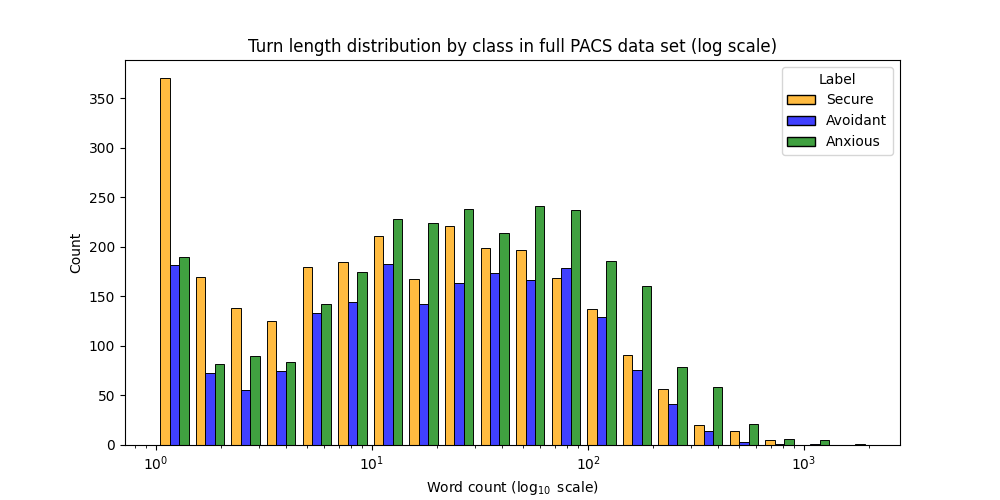
\includegraphics[width=\textwidth]{figures/log_dodge_turn_length_distribution_by_class.png}
    \caption{Distribution of patient speech turn length per class.}
    \label{fig: class balance turn len}
\end{figure}

\subsection{Approach}
To begin development on the classification model, the data is split into 85 \% training and 15 \% test data.
This split was chosen to allow the model as much data as possible for training, given the low amount of available data overall.
The split was performed with stratification according to class balance, a measure necessitated by the low amount of documents.
It is important to split at the document level to avoid data leakage and ensure that the model is not learning to recognise individuals but rather generalisable speech patterns according to PACS classification.
The relatively small amount of samples in the test set is somewhat made up for by applying cross-validation and reporting a mean accuracy for all models of the best performing configuration.
All models were implemented using the Massive Choice, Ample Tasks (MaChAmp) framework for transfer- and multi-task learning developed by van der Goot et al. \citeyear{MaChAmp}, which itself relies on the HuggingFace Transformers library \cite{HuggingFace} and PyTorch \cite{PyTorch}.
The source code for this project is available at \url{https://github.com/Fred-Bred/PACS-AI}.

\subsubsection{Domain-Adaptive Pre-Training}
To investigate whether models could learn more task-appropriate representations from being exposed to more unlabelled data from the task domain, I conducted domain-adaptive pre-training with both a RoBERTa-base model \cite{roberta} and the pre-trained MentalRoBERTa model presented by Ji et al. \citeyear{MentalBERT}.

In domain-adaptive pre-training, the base language model undergoes continued training on domain-relevant unlabelled data.
Text is considered domain-relevant if it concerns topics relevant to the task, is of a relevant genre, or originates from forum discussing the topic.
Training is done on masked language modelling objective (i.e., cross-entropy loss on predicting randomly masked tokens).
This type of training has been found to consistently improve performance of RoBERTa on classification tasks in low-resource settings \cite{Gururangan2020}.

\paragraph*{Domain data}
The domain data used for pre-training came from three different datasets.

First, the AnnoMI dataset \cite{Wu2022}, which consists of professionally transcribed and annotated dialogues of both high- and low-quality motivational interviewing.
Motivational interviewing is an effective form of counselling for habit- and behaviour change \cite{Apodaca2014, Gillam2019}.
A 2005 review also found it to be beneficial in various behaviour change contexts and found clinically relevant benefits for both physiological and psychological diseases \cite{Rubak2005}.
From this dataset 4,817 client utterances were extracted for use in pre-training.
Setting aside 20 \% of instances to validate the model during training leaves 91,479 tokens for pre-training.

Second, the DAIC-WoZ dataset \cite{Gratch2014}, consisting of 275 transcripts of clinical interviews, between seven and 33 minutes in duration, conducted by an animated virtual interviewer controlled by a human interviewer in a different room.
Because the annotation of this dataset can at times be ambiguous with regard to who is speaking, all utterances were included in the pre-training data.
This resulted in a total of 26,083 utterances. As above, setting aside 20 \% of samples for validation leaves 371,089 tokens for pre-training.

Finally, the HOPE dataset \cite{Malhotra2022} is made up of 212 counselling transcripts collected from various publicly available sources from which 6,382 patient speech turns were extracted for pre-training.
148,109 tokens were kept for pre-training.

While other data sources are available, these tend to be either significantly lower quality or of limited relevance.
For instance, a number of large datasets have been constructed from text that is supposedly relevant to models in the mental health domain, such as tweets labelled with emotional valence (e.g., tweeteval; \citeNP{tweeteval}, used by \citeNP{Wagner2023}), Reddit posts related to mental health topics \cite{Kim2020, MentalBERT}, or chat forums on psychological counselling \cite{counselchat}.
These, and similar entirely text-based datasets, were deemed too far removed from the language and nuance of spoken in-person therapy.
Nevertheless, one encoder pre-trained on Reddit data (MentalRoBERTa; \citeNP{MentalBERT}) was included in the experiments to test this assumption.

\paragraph*{Pre-training approach}
For each of the pre-training datasets, 20 \% of the utterances were kept from the model during training as a development set.
All the remaining data from all three datasets where combined in a single raw text file to train on.
I applied an approach similar to the RoBERTa training methodology.
This includes dynamic masking, where each token is masked with probability 0.15 and the model is exposed to each sequence on several occasions during training.
Despite this not being implemented in MaChAmp \cite{MaChAmp}, I deemed it to be necessary due to the relatively low amount of data for masked language modelling.
Additionally, as prescribed by Gururangan et al. \citeyear{Gururangan2020}, only the masked language modelling objective was used.
Following recommendations from MaChAmp documentation, I duplicated the training data four times, leaving me with a training dataset five times the original size.
Each model trained on this data, consisting of a total of 3,053,385 tokens (610,677 before duplication), for 20 epochs, seeing each sample once, and evaluating perplexity on the development set after each epoch.
With five copies of the training data, this corresponds to training five epochs with a more frequent evaluation strategy.

Nevertheless, the best model, as determined by the validation set performance on the MLM task, was consistently the first of 20.
This is curious as the model at this point has yet to see all the unique samples.
This might suggest that not enough pre-training data was made available for the approach to have the expected results or that this domain is particularly difficult to adapt to.

\subsubsection{Target Task Fine-Tuning}
Hyperparameter values were chosen based on what had been previously demonstrated to work well for similar applications and on the basis of both theory and experiments.
Experiments for hyperparameter tuning were run by training on 85 \% of the training data and tracking the training progress by tracking metrics on the remaining 15 \%.

Once hyperparameters were fixed, experiments centred around preprocessing methods and comparing different encoders.

\paragraph*{Inputs and batching}
All models were initialised with their maximum input length of 512 tokens.
Due to the low amount of data available, increasing maximum input length did not meaningfully impact computation requirements.
Additionally, the task data contains sequences of varying length, some of which reach or even exceed this limit.

Following several unstable runs with batches of 16 samples, batch size was increased to 32 for all models, which appears to provide a good balance of frequent gradient updates and stability in training.
During training, batches are shuffled between epochs, such that each epoch presents new combinations of samples to the model.

\paragraph*{Learning rate schedule}
Following experiments, a base learning rate of $1 \times 10^{-5}$ was selected.
While a learning rate of $5 \times 10^{-5}$ was found by Sun et al. \citeyear{Sun2020} to work well for text classification tasks with similar types of pre-trained models, experiments with this and higher base learning rates produced unstable training, while lower learning rates generally produced poorer metrics, likely as models would be unable to escape local minima.

A slanted triangular learning rate schedule is implemented similar to the formulation by Howard and Ruder \citeyear{Howard2018}, albeit with slightly different values.
This schedule implements a linear warm-up for a specified fraction of the training steps, here, 0.3, before linearly decreasing the learning rate over the remaining steps, referred to as annealing.
This method is implemented with a ratio of 32 as the difference between the smallest and base learning rates.
Additionally, gradual unfreezing and discriminative fine-tuning are implemented.
Gradual unfreezing refers to a method in which training begins by adjusting only the classification head, keeping the encoder constant.
Once the first epoch has been completed, the second-to-last layer in the model is unfrozen and adjusted during the second epoch.
This process continues until all layers are unfrozen and actively being adjusted.
During the unfreezing process, the learning rate is cyclically increased and annealed according to the slanted triangular schedule within each epoch.
Once all layers have been unfrozen, the learning rate is increased and annealed over all remaining training iterations.
Discriminative fine-tuning slightly adjusts this process such that when a layer is first unfrozen, it is trained with a lower learning rate than the rest of the model.
Discriminative fine-tuning is implemented here with a decay factor of 0.38, by which the learning rate of newly unfrozen layers is decreased.

\paragraph*{Optimisation and regularisation}
Both fine-tuning and masked language modelling are done using a cross-entropy loss.

Optimisation is performed using the AdamW algorithm introduced by Loshchilov and Hutter \citeyear{AdamW}.
This algorithm applies the classic Adam optimiser \cite{Adam} with weight decay.

Additionally, dropout is applied with probability 0.2.
During training, dropout randomly sets a proportion of activations within the network to zero at each forward pass.
This technique encourages the model to learn robust features, preventing overfitting by reducing reliance on specific weights for decision-making.

\subsubsection*{Experiments}
\paragraph*{Turn length}
I hypothesised that the very short sequences of e.g. less than five words, would be less informative for the model.
To test this hypothesis, I first tracked performance over different input sequence lengths during the early experimentation.
For the majority of test, this did not confirm my initial hypothesis, and, in fact, many models exhibited their best performance on the very short sequences.
See Figures \ref{fig: acc over turn len 7} and \ref{fig: acc over turn len 11} in Appendix \ref{App: Figures} for an example of a plot of one such experiment.
I suspected that this was because the classes were less balanced in this portion of the dataset.
Findings by Daniel \citeyear{Daniel2011} and Miller-Bottome et al. \citeyear{MillerBottome2018}, as reported in section \ref{sec:Differentiable approaches}, would suggest that avoidant patients should be overrepresented here, if they primarily use short speech turns.
However, if they generally take fewer speech turns, they may be underrepresented in all counts.
Figure \ref{fig: class balance turn len} in Appendix \ref{App: Figures} reveals that, in fact, the class balance in the short speech turns varies substantially from the distribution in the full dataset.
In the very short speech turns, secure patients are overrepresented compared with their share of total transcripts but, somewhat surprisingly, the two other classes are represented roughly as expected from their overall contribution to the dataset.

It is not clear how the shifting class balance over turn lengths influences the models' ability to differentiate classes or to learn generalisable patterns.
To investigate whether models would benefit from seeing only longer sequence of patient speech I conducted preprocessing experiments in which I would define a minimum speech turn length, measured in word count, and combine speech turns within documents until the minimum count had been reached.
I ran these experiments with minimum turn lengths of 50, 100, 150, and 250 words.
In these experiments, each client speech turn is included in the dataset as-is if it is at or above the defined minimum.
If it is below the threshold, it is combined with the following speech turn in the same document and then checked again, where the same rule is applied.
The final speech turn in each document is included only if it meets the threshold alone or if it has already been combined with (a) previous turn(s).

\paragraph*{Encoders}
The pre-trained model which encodes the input sequence before passing it on to the classification head can massively impact the performance of the model.
This encoder represents almost the entirety of the model and the parameters to be adjusted during training.
To optimise for the best suited encoder in the RoBERTa species, I tested five different encoders.
The first two are the base and large versions of the RoBERTa model originally trained by Liu et at. \citeyear{roberta}.
The three remaining models are all domain-adapted to some degree.
First, the base size MentalRoBERTa model trained by Ji et al. \citeyear{MentalBERT}.
This model is an instance of the base RoBERTa model which has been further trained on Reddit posts related to mental health on the masked language modelling objective.
In theory, this might make the model and its embeddings more attuned to patterns related to mental health and themes related to psychotherapy.
Finally, as described above, I conducted my own pre-training of a base RoBERTa model as well as continued domain-adaptive training of the MentalRoBERTa model.

\paragraph*{Grid search and cross-validation}
Following early experiments, validation results were observed to be rather unstable during training.
In order to obtain more reliable results and to better determine the best configuration of encoder and minimum input length, I performed a grid search with five-fold cross-validation through each combination of the selected encoders and minimum input length.
Five-fold cross-validation is a method of obtaining more reliable results in which the training data is split into training and validation data five different times, producing five different splits.
Different models are trained and validated on each split, and the final result is the mean of the validation performance across folds.
This result is used to determine the best configuration (i.e., combination of encoder and minimum input length) which can then be applied to the test set in a similar fashion.
With five encoders and five minimum lengths to search over, five-fold cross-validation resulted in 125 models to train.
As the available computational resources were somewhat limited, I opted to not test any larger models, nor to include grid-search over other hyperparameters.

\section{Results}
Validation results in the form of mean and standard deviation accuracy for each encoder and minimum input length combination are displayed in Table \ref{tab: val results}.
The efforts to produce domain-adapted models do not seem to have been helpful for this task.
This is the case for both my own pre-training and when using a domain-specific model (MentalRoBERTa; \citeNP{MentalBERT}) as well as for my further pre-training of the domain-specific model.

Additionally, providing the model with more context per sample by increasing the minimum input length seems to improve performance in most cases.
However, albeit less consistently, it also tends to increase instability.
This is undoubtedly due to the lower number of instances available in the validation set when more sample must be combined to reach a longer minimum length.
\begin{table}
\begin{adjustbox}{width=1\textwidth}
    \begin{tabular}{lrrr}
\toprule
Encoder & Minimum turn length & Mean validation set accuracy & Standard deviation \\
\midrule
\multirow{5}{*}{RoBERTa-base} & 0 & 45.28 & 7.21 \\
& 50 & 47.37 & 5.47 \\
& 100 & 51.99 & 7.42 \\
& 150 & 51.78 & 4.27 \\
& 250 & 59.86 & 9.67 \\
\midrule
\multirow{5}{*}{RoBERTa-large} & 0 & 49.27 & 3.40 \\
& 50 & 48.84 & 5.40 \\
& 100 & 54.88 & 6.94 \\
& 150 & 56.15 & 5.21 \\
& 250 & 58.67 & 11.64 \\
\midrule
\multirow{5}{*}{MentalRoBERTa} & 0 & 46.79 & 7.82 \\
& 50 & 50.65 & 6.49 \\
& 100 & 54.90 & 5.51 \\
& 150 & 53.69 & 5.31 \\
& 250 & 58.89 & 6.01 \\
\midrule
\multirow{5}{*}{Pre-trained RoBERTa-base} & 0 & 45.17 & 6.70 \\
& 50 & 48.84 & 4.97 \\
& 100 & 49.16 & 8.66 \\
& 150 & 51.75 & 5.38 \\
& 250 & 59.40 & 7.68 \\
\midrule
\multirow{5}{*}{Pre-trained MentalRoBERTa} & 0 & 47.30 & 5.00 \\
& 50 & 50.44 & 7.20 \\
& 100 & 54.57 & 9.59 \\
& 150 & 51.93 & 6.54 \\
& 250 & 57.22 & 9.47 \\
\bottomrule
\end{tabular}

\end{adjustbox}
\caption{Validation results}
\label{tab: val results}
\end{table}

% \begin{tabular}{lrrr}
%     \toprule
%     Encoder & Minimum turn length & Mean validation set accuracy & Standard deviation \\
%     \midrule
%     \multirow{5}{*}{RoBERTa-base} & 0 & 45.28 & 7.21 \\
%     & 50 & 47.37 & 5.47 \\
%     & 100 & 51.99 & 7.42 \\
%     & 150 & 51.78 & 4.27 \\
%     & 250 & 59.86 & 9.67 \\
%     \midrule
%     \multirow{5}{*}{RoBERTa-large} & 0 & 49.27 & 3.40 \\
%     & 50 & 48.84 & 5.40 \\
%     & 100 & 54.88 & 6.94 \\
%     & 150 & 56.15 & 5.21 \\
%     & 250 & 58.67 & 11.64 \\
%     \midrule
%     \multirow{5}{*}{MentalRoBERTa} & 0 & 46.79 & 7.82 \\
%     & 50 & 50.65 & 6.49 \\
%     & 100 & 54.90 & 5.51 \\
%     & 150 & 53.69 & 5.31 \\
%     & 250 & 58.89 & 6.01 \\
%     \midrule
%     \multirow{5}{*}{Pre-trained RoBERTa-base} & 0 & 45.17 & 6.70 \\
%     & 50 & 48.84 & 4.97 \\
%     & 100 & 49.16 & 8.66 \\
%     & 150 & 51.75 & 5.38 \\
%     & 250 & 59.40 & 7.68 \\
%     \midrule
%     \multirow{5}{*}{Pre-trained MentalRoBERTa} & 0 & 47.30 & 5.00 \\
%     & 50 & 50.44 & 7.20 \\
%     & 100 & 54.57 & 9.59 \\
%     & 150 & 51.93 & 6.54 \\
%     & 250 & 57.22 & 9.47 \\
%     \bottomrule
% \end{tabular}

It is my assessment that the model configuration that provides the optimal balance between performance and stability is the RoBERTa-large variant with a minimum input length of 150 words, performing at an average accuracy of 56.15 \%.
The RoBERTa-large model appears to hold the greatest promise out of the encoders tested, perhaps suggesting that larger models with greater capacity should have been included in the tests.
The RoBERTa-large encoder will be the centre of the remaining analysis, focusing primarily on the 150 words minimum input length variant.

Following cross-validation, five instances of the RoBERTa-large model were saved.
Taking a majority vote between the five models to determine one prediction per sample in the test set produced the confusion matrix in subplot A of Figure \ref{fig: all confusion matrices}.
% $$
% \begin{bmatrix} 3 & 0 & 19 \\ 0 & 4 & 8 \\ 2 & 0 & 53 \end{bmatrix}
% $$
Subplot B to F display the confusion matrices for each instance of the model.
Full size confusion matrices for each of the five individual models are included in Appendix \ref{App: confusion matrices}.
The mean test set accuracy across these five models is 59.55 \% with a standard deviation of 5.82.
Metrics for each model are reported in table \ref{tab:roberta-large_150 test metrics}.
The accuracy score of the ensemble voting classifier using all five instances of the RoBERTa-large model is 67.42 \%.

\begin{table}
    \begin{adjustbox}{width=1\textwidth}
        \begin{tabular}{lrrrrr}
    \toprule
    Model & Accuracy & Precision & Recall & F1-score & $\kappa$ \\
    \midrule
    Split 1 & 60.67 & 37.30 & 34.55 & 30.07 & 0.03 \\
    Split 2 & 68.54 & 61.42 & 63.79 & 62.09 & 0.41 \\
    Split 3 & 51.69 & 42.10 & 47.98 & 41.50 & 0.17 \\
    Split 4 & 61.80 & 37.45 & 35.15 & 30.37 & 0.04 \\ 
    Split 5 & 55.06 & 44.86 & 44.81 & 43.17 & 0.12 \\
    \midrule
    Mean & 59.55 & 44.63 & 45.26 & 41.44 & 0.15 \\
    Ensemble & 67.42 & 75.42 & 47.78 & 50.25 & 0.23 \\
    \bottomrule
\end{tabular}
    \end{adjustbox}
    \caption{Test set metrics for each instance of the RoBERTa-large model trained with minimum input length of 150 Words. Precision, recall and F1-scores are macro-averaged.}
    \label{tab:roberta-large_150 test metrics}
\end{table}

\begin{figure}
    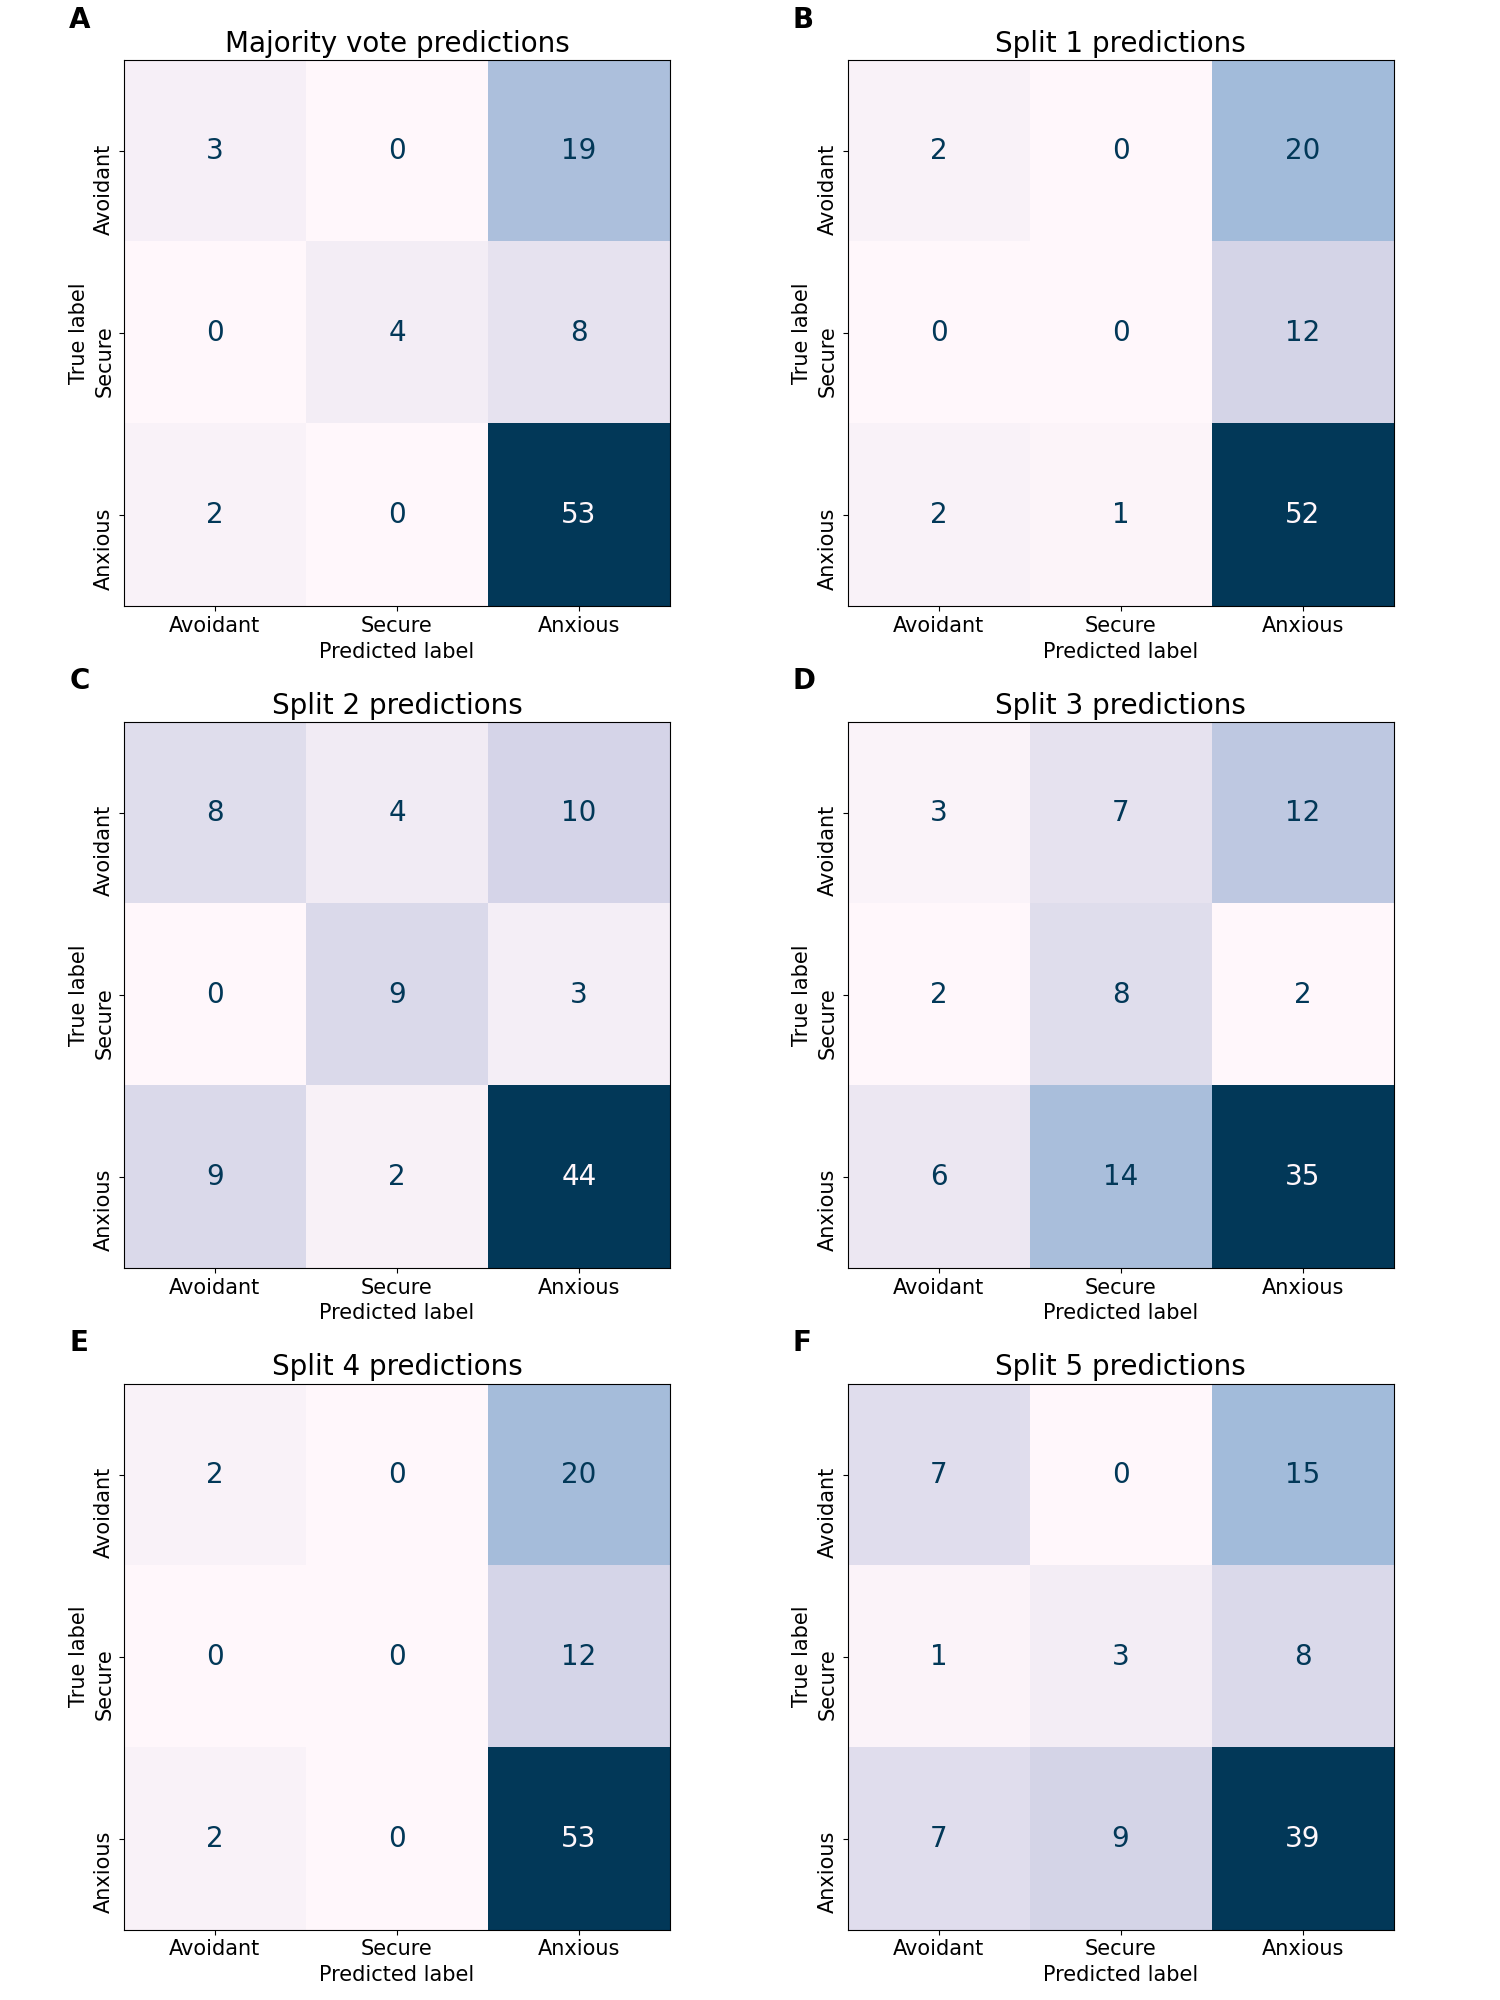
\includegraphics[width=0.95\textwidth]{figures/combined_confusion_matrix.png}
    \caption{Confusion matrix for the majority vote predictions and each of five iterations of RoBERTa-large trained with minimum input length of 150 words.}
    \label{fig: all confusion matrices}
\end{figure}

\section{Discussion}
In this thesis, I set out to assess the feasibility and utility of automatically classifying patients' attachment characteristics during psychotherapy.

It is clear that the models heavily weight the anxious class, a preference somewhat justified by the skewed distribution in both training and test sets using this preprocessing method.
The training set class distribution when speech turns are concatenated to reach a length of at least 150 words is as follows:
\begin{itemize}
    \item Avoidant: 20.70 \%
    \item Secure: 31.63 \%
    \item Anxious: 47.67 \%
\end{itemize}

It should be noted that while the ensemble confusion matrix presents heavily skewed towards an over-reliance on the majority class, the same degree of skewness is not present in all instances of the model.
However, a closer look at the classification patterns of the models is warranted.
In the therapy setting, the most trivial error would likely be to confuse a secure patient for being either type of insecure.
As covered in section \ref{sec:Differentiable approaches}, secure patients may be better able to profit from treatment regardless of the specifics of its organisation.
Confusing either of the insecure orientations for being secure is likely to lead to worse outcomes as therapists may alter their strategies for building the therapeutic alliance and structuring the course of treatment in counterproductive ways.
However, this error may be less severe for avoidant patients, as the association between this orientation and therapy outcomes is weaker while this group of patients tend to hold more stable views of their therapists and working alliance (see sections \ref{sec: Health} and \ref{sec:Applying attachment in therapy}).
Most dire are the consequences of confusing the two insecure attachment patterns.
If a therapist were to follow the prescription by Slade \citeyear{Slade2016} by structuring the course of their treatment and approaching the alliance building process according to the attachment characteristics of the patient, doing so on the basis of a misclassification could be detrimental.
The approaches suggested to align best with these two attachment patterns are almost exactly mirrored, risking serious adverse outcomes from the misguided structuring of treatment according to a misclassification.

Given that the three-class problem corresponds to a flattening of the two-dimensional space described by the dimensions of anxiety and avoidance, one would expect any capable classifier to most easily distinguish the extremes of the scale, i.e., between anxious and avoidant patients.
However, this does not appear to be the case, as these two classes are frequently confused across all five models.
Namely, across the five models, the two insecure classes tend to be confused as often or more often than the secure class is confused with either of the insecure classes.
Referencing the ensemble confusion matrix, the avoidant patients are recognised with the greatest difficulty.
In fact, this ensemble model achieves only a recall of 13.64 \%, indicating that the vast majority of avoidant patients are misclassified.
Due to the bias for anxious classification in most models, in the ensemble classification, the mislabelled avoidant patients are instead classified as anxious.

% Not sure if this should go here? Could maybe go in future directions in the bit where I also talk about capacity and data?
The ensemble of all five models produces higher accuracy, precision, recall, and F1-scores than the majority of individual models and these scores are above the mean for each metric.
Consistently outperforming the majority of models may suggest that individual models, trained on different portions of the data, have learned to represent different aspects of the problem.
This could indicate that models have not converged on the similar representations that one would expect.
This effect of data split indicates that these models may be able to learn more robust representations with access to more data.
Similarly, greater capacity, i.e. larger models, may enable models to simultaneously represent the various features that the different models have prioritised.

To further investigate the impact of affording the model more context, Figure \ref{fig: roberta-large results} displays the mean test set accuracy and standard deviation for RoBERTa-large models across minimum input lengths.
While it is not custom to run several models on the test set, I do so sparingly in this project to demonstrate the effects of additional context, which may provide direction for future research and development.
As hypothesised, adding context to the very short speech turns tends to improve performance.
However, it comes with a noticeable trade-off of stability as both training and testing sample sizes decrease and standard deviations in mean accuracy scores tend to increase.
This seems to suggest that with a larger dataset, the model would have more opportunity to encode the relevant information required to predict attachment style by increasing the information and context available to it.

\begin{figure}
    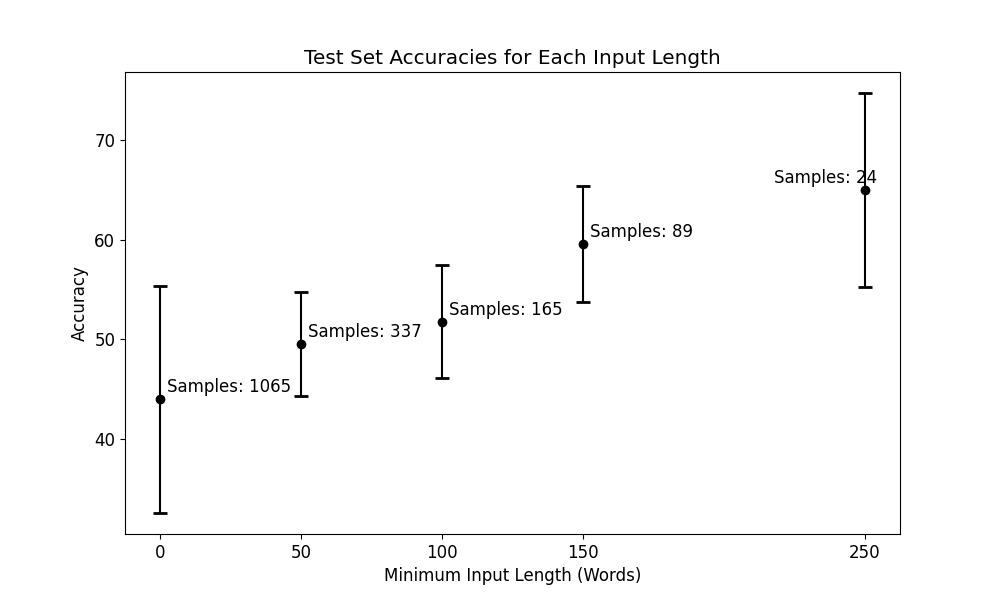
\includegraphics[width=\textwidth]{figures/roberta-large_acc_for_min_len.png}
    \caption{Mean and standard deviation accuracies in test set for all models resulting from five-fold cross-validation over varying minimum input lengths. Error bars represent one standard deviation.}
    \label{fig: roberta-large results}
\end{figure}

This manner of concatenating speech turns to reach a minimum word count has an unintended side effect.
Namely, the distribution between the three classes changes as more speech turns are concatenated.
Unfortunately, the relatively small datasets mean that this effect is not uniform across training and test splits.
Rather, in the test split, concatenating to at least 150 words results in an increased skew and in swapping the size rankings of the secure and avoidant classes:
\begin{itemize}
    \item Avoidant: 24.72 \%
    \item Secure: 13.48 \%
    \item Anxious: 61.80 \%
\end{itemize}

This skewed distribution challenges the interpretation of the above results as demonstrating the beginning of learning to distinguish classes.
In fact, the majority of models do not perform above this new majority baseline.
In spite of this, I am optimistic that the models have generally learned to encode some relevant information for distinguishing the three classes.
While several models do not improve in accuracy over the majority baseline, the ensemble model does.
Additionally, based on the distribution in the larger training dataset, I believe that the majority baseline in the test set is, in a sense, artificially high.
While a robust well-performing model would not necessarily struggle with this distribution, it does set a somewhat inflated baseline for comparison.

\subsection{Implications}
Clinical judgement is a complicated and subjective task and tends to produce far from perfect inter-rater agreement.
The results of this thesis must be viewed not only in light of the low amounts of data available but also with the broader difficulties involved in clinical judgement in mind.
To provide a fitting frame of reference, I will briefly review some data on the reliability of expert and clinical judgement in psychology, before considering the implications of this project.

Very recently, Wagner et al. \citeyear{Wagner2023} found 76-80 \% inter-rater overlap for evaluations of mental health status when different experts rated the same samples in their dataset of psychotherapy text.
While this is generally considered good inter-rater agreement, Wagner et al. also point out how it highlights the subjective nature of psychological evaluations.

Inter-rater agreement on psychiatric diagnosis tends to be quite high when patients are assessed through structured interviews.
Ruskin et al. \citeyear{Ruskin1998} reported a mean $\kappa$ of .83 for major depression, bipolar disorder, panic disorder, and alcohol dependence when assessed using a structured clinical interview.
Psychotic disorders, however, tend to have substantially lower agreement between raters.
For instance, Maj et al. \citeyear{Maj2000} found only $\kappa = .22$ for schizoaffective disorder, while the affective disorders manic and major depressive episodes produced $\kappa$ of .71 and .82, respectively.

In a study of 217 psychiatric consultations, Al-Huthail \citeyear{Al-Huthail2008} found that the accuracy of initial psychiatric impression by primary medical providers when compared with final psychiatric diagnosis was just 60 \% for cognitive disorders, 50 \% for depression and 46 \% for anxiety disorders.

Considering more directly the reliability of the gold standard attachment measure, the adult attachment interview (AAI) has produced remarkably high inter-rater agreement and test-retest reliability scores.
For instance, Sagi et al. \citeyear{Sagi1994} found 90-100 \% agreement between their raters on three-way classification (secure, anxious, avoidant) of their AAI transcripts ($\kappa = .82 - 1.0$ for comparisons between three raters). Their test-retest agreement across raters was 90 \% ($\kappa = .79$).
Similarly, Bakermans-Kranenburg and van IJzendoorn \citeyear{BakermansKranenburg1993} found test-retest reliability for three-way classification of the AAI of 78 \% ($\kappa = .63$).
More recently, Talia et al. \citeyear{Talia2020} found an inter-rater agreement of .88 on their test of a small sample of interviews coded according to the AAI manual.

Even in the absence of directly comparable measures, it is clear that human expert raters generally fare better than the models presented here, albeit with their own limitations.
However, this edge in performance must be considered in light of the additional information available to human raters.
Depending on the task, these experts may have the option of asking follow-up questions, and they typically work with much greater context.
For instance, when classifying an AAI, the rater has access to the entire transcript at once.
This allows not only for the analysis of long-term patterns in speech and behaviour but also for inclusion of relevant context such as the therapist or interviewer speech turns, which were not made available to models in this project.
These affordances highlight that the target for an automated assessment system is not perfect reliability, but rather to reliably reach or exceed the human baseline for comparable tasks.
In spite of the somewhat lacklustre results of the models presented here, I believe that the present results -- achieved with limited data and models of moderate size -- demonstrate that automated decision support of the kind that this thesis begins to develop may achieve this in the near future.

The high reliability of structured psychiatric interviews as well as both the PACS and the AAI and the comparatively low reliability of unstructured clinical judgement suggests that conducting clinically relevant judgement of psychological phenomena in one's patients is an exceedingly difficult task.
These issues are not unrecognised by psychiatrists, and Matuszak and Piasecki \citeyear{Matuszak2012} suggest that more structured approaches be applied to both the anamnesis and diagnosis processes.
Exacerbating the issue, it seems likely that in the somewhat unstructured psychotherapy dialogue in which the therapist's emotional and cognitive resources are likely to be focused elsewhere, the task of accurately assessing a patient's psychological characteristics becomes increasingly difficult.
As such, rather than relying entirely on the intuitive judgement of therapists who may need to direct their focus elsewhere, I suggest that qualified decision support is warranted.
Machine and clinical judgement does not have to be a dichotomy.
In fact, a union is not only legitimate but justified, given adequate performance in the future.
In the ideal case, an automatic decision-support system for the assessment of attachment orientation can free up therapists' resources and allow them to be more present in their counselling sessions while providing more accurate and reliable repeated measurements for research and to inform treatment and intervention design.

For the purpose of psychotherapy research, existing methods tend to either lack reliability as repeated measurements as individuals become accustomed to the interview procedure (AAI; \citeNP{Daniel2015}) or offer questionable validity due to the superficial nature of self-report measures \cite{Talia2017}.
The method explored here offer a future solution to this problem as such a tool could deliver reliable and valid repeated measures to track attachment characteristics over time.

\subsection{The Ethics of Automated Analysis}
When applying any automated process, the potential for bias is always a serious concern.
In the case of using language models in psychological research and practice, Demszky et al. \citeyear{Demszky2023} point to two primary sources or types of harm arising from bias.
First, representational harms can arise when some groups are represented by the outputs of generative models or in the embeddings of discriminative models in unfavourable ways.
Second, allocational harms may arise when algorithms are employed in distributing resources (e.g. loans, access to therapy) but do so differentially according to biases present in the training data.

While attachment behaviours are theoretically expected to be very similar across cultures, owing to their theorised evolutionary and biological basis, their exact verbal expression may vary across cultures and socio-economic divides.
As such, differences may exist that the model is poorly equipped to learn based on both its original training data and the somewhat homogeneous task data.
This may lead this and other models to systematically mislabel patients of different demographics than those of the majority of their training data.
It is essential for progress in the combined field of natural language processing and psychotherapy that the generation of future datasets involve representatives from the communities meant to be served by the products.
The approach presented in this thesis protects the users to some extent by maintaining the therapist as the decision-maker, acting entirely as a complimentary tool or decision support, but ultimately leaving it up to each therapist to apply their own judgement in shaping the course of treatment.
Nevertheless, the impact of machine-generated classifications on clinical judgement can be enormous and therapists working with these types of tools should be educated on how to interpret their outputs.
Such training should equip therapists to avoid undue influence and bias from the model.

In their analysis of over 10,000 adult attachment interviews, Bakermans-Kranenburg and van IJzendoorn \citeyear{Bakermanskranenburg2009} found a striking lack of influence from gender, language, and culture on the overall distribution of attachment classification.
This suggests that the core dimensions of attachment behaviour might be more universal than most psychological constructs.
However, it is important to distinguish this from universality in expression.
Cultural variations in how attachment styles are manifested and expressed through cues in language might still exist, even if the underlying constructs are similar.
Overall, however, these findings support the potential applicability of machine learning approaches to attachment assessment across cultures.

The issue of interpretability and transparency in decision-making remains an important consideration to be balanced with performance objectives.
In all cases where outputs directly influence decisions related to the classification or treatment of individuals, interpretability is a priority.
With the current state of explainability research in NLP, this remains irreconcilable with useful degrees of predictive reliability (see e.g., \citeNP{Danilevsky2020, BarredoArrieta2020}), thus highlighting the importance of leaving decision competence with well-trained therapists supported by reliable tools providing useful insights rather than outsourcing it entirely to algorithms.

While the present results do not represent a tool ready for clinical deployment, they show the potential of these methods for broader application.
The most appropriate application at this stage of maturity is in research.
Here, large-scale projects can leverage the efficiency of automating classification while alleviating the individual consequences of potential misclassifications.
This may enable research projects at all scales to develop knowledge on and strategies for managing attachment insecurity and how it affects the therapeutic process.

\subsection{Limitations and Future Direction}
The primary challenge to the investigation of the utility and feasibility of automatic classification in this domain is the low amount of data available.
Due to the sensitive nature of therapy transcripts, the collection and sharing of large corpora of transcripts is both ethically and logistically challenging.
This project was severely limited by only working with 78 transcripts in total, and I believe that future work, should it succeed in gathering larger and more diverse corpora of relevant texts, would likely produce more impressive classification results that what has been demonstrated here.
Furthermore, this project may have been hampered by its stratification strategy.
As the split between training and test data was made at the document level to avoid data leakage, this is also the level at which stratification was considered.
However, in spite of the initial stratification, this produced training and test sets with vastly different class distributions after the extraction and concatenation of speech turns.
To combat this, future projects may experiment with more sophisticated stratification strategies for producing training and test splits.
Once follow-up projects have more accurately determined the optimal balance between number of samples and context per sample, test and training splits can be made at the document level while stratifying for class distribution at the level of (concatenated) speech turns.

This project has tested language models of moderate size. All base RoBERTa models have roughly 125M parameters while the large variant has approximately 355M parameters.
Considering the increasing availability of Large Language Models (LLMs), there may be other feasible approaches for this type of classification.
Larger models theoretically have more potential for learning complex dependencies and recognising abstract patterns of behaviour.
In this project, the largest model tested produced the most convincing validation results, indicating that more capacity may be appropriate for this task.
However, this increased capacity tends to also express itself as an increased capacity for overfitting.
This becomes a particularly serious concern when one considers the comparatively minuscule datasets that tend to be available in this field as was the case in this project.

The models applied in this project were developed in 2018. Newer text processing models have substantially larger context windows and in the near future, some models may be able to process entire transcripts at once, considering all speech turns and interactions.
Doing so may allow models to consider context in the form of therapists' contributions to the conversations which may provide valuable information given the capacity to incorporate it.
Beyond the simple addition of more high-quality labelled data, this may prove to be the necessary intervention in closing the gap between machine and human judgement on abstract psychological constructs such as attachment.
Even in this small dataset, considering only patient speech turns, adding more context in the form of a longer minimum input generally produced better accuracy.
Moreover, the fact that the larger models tended to produce the best results when both performance and stability are considered opens an obvious avenue of research into applying models with greater capacity once larger datasets become available.

Continuous -- rather than categorical -- measures of attachment may be considered both more theoretically congruent and empirically more appropriate and thus be preferred.
Future work should attend to this fact and work towards integrating it in the continued development of these types of methods.
This may be done by e.g. tagging individual PACS discursive markers in transcripts or developing models to directly score the subscales given measures from the PACS or AAI.
Because continuous measurements were not available at the development of this project, it aims instead to provide a proof of concept for the automatic classification of attachment using the categorical convention.
Nevertheless, the study of in-session behaviour remains so highly relevant that its primary counterarguments arguably lie in the feasibility and scalability domains.
The benefits to clinical practice, as outlined in section \ref{sec:Applying attachment in therapy}, are numerous.
Of equal importance is the interest in and methods enabling investigation of in-session behaviour and its relevance to clinical outcomes which may enable further research that will transform the practice of psychotherapy and therapist training programmes.
Talia et al. \citeyear{Talia2017} point out that studies using the PACS can move beyond exploring the link between attachment and treatment outcomes and investigate associations between \textit{changes} in attachment and treatment outcomes.
Additionally, the notion of tracking in-session behaviour over time and associating it with therapist behaviours and interventions offers a promising and potentially impactful branch of research \cite{Slade2016, Talia2017}.
This thesis begins the work of addressing the feasibility challenge by automating the classification task.
In the future, this will enable scalable pipelines for research and clinical practice in which automatic speech recognition (a fast developing area in automated data processing) can feed into models such as the one presented here for classification or continuous assessment.

\section{Conclusion}
Attachment characteristics affect great influence over important aspects of every day life, health outcomes, and the treatment effects and strategies of psychotherapy.
However, its assessment is a time-consuming procedure, which risk losing validity upon close repetition \cite{Daniel2015,Hesse1999}.
The Patient Attachment Coding System (PACS) enables repeated and nonintrusive assessment in the natural context of psychotherapy and offers an explainable link between patient speech patterns and attachment classification \cite{Talia2017,Talia2014}.
The PACS offer invaluable theoretical insight but is similarly time-consuming to learn and apply.

As such, the prospect of automating the assessment of attachment characteristics in psychotherapy holds great value for both research and practice.
This thesis investigated the feasibility of one method for automating this assessment.
Based on a small dataset collected as part of a PACS validation study \cite{Talia2017}, a variety of RoBERTa models \cite{roberta} were fine-tuned to predict the PACS classifications of psychotherapy patients from as little context as a single patient speech turn.

Almost all models perform above the random baseline.
Test set predictions for cross-validation instances of the same model configuration beat the majority baseline when model instances are applied as a voting classifier, in spite of most of the single model instances not beating the test set majority baseline.
This and further analysis provide initial but tentative support for the method despite unimpressive classification accuracy.

Future work should aim to apply newer and larger models, more sophisticated stratification and training strategies, and, most importantly, larger datasets to begin approaching performance that would enable the deployment of these models.
Deployment should begin in research were individual consequences of misclassification are mitigated by aggregation and application.

\bibliography{references}

\appendix
\chapter{Figures}
\label{App: Figures}

\begin{figure}
    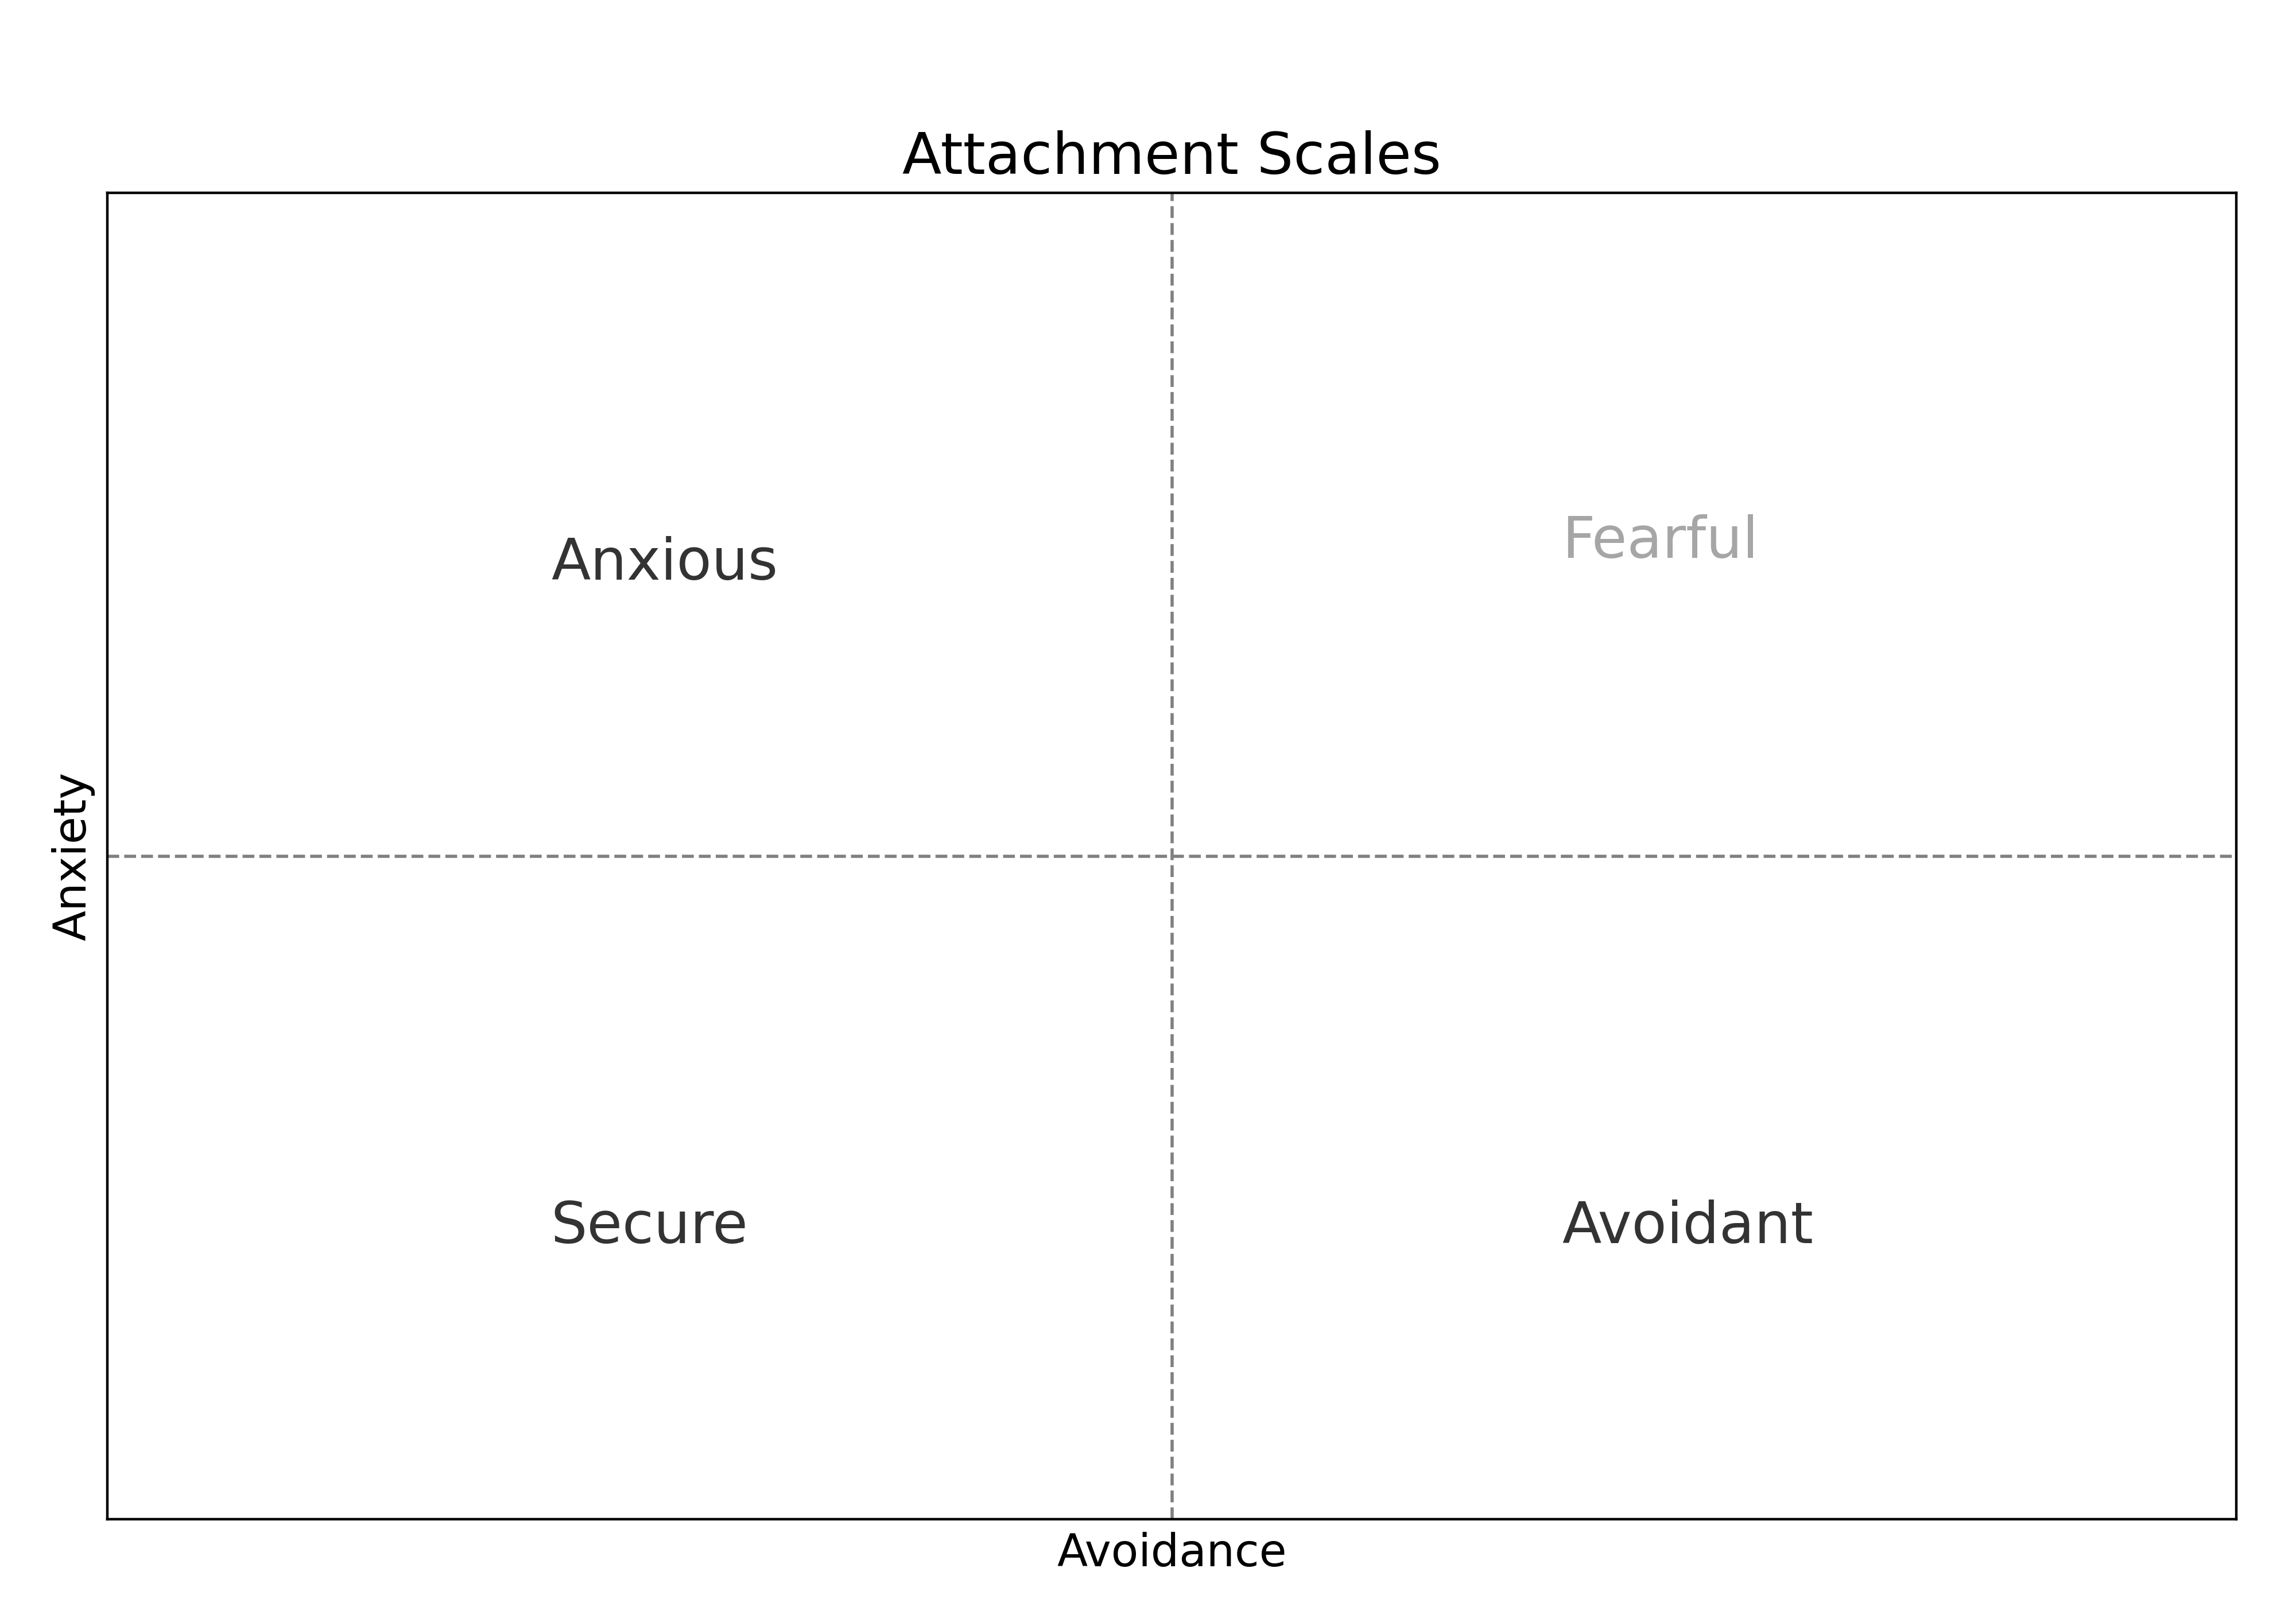
\includegraphics[width=\textwidth]{figures/attachment_scales.png}
    \caption{The two orthogonal scales of anxiety and avoidance visualised.}
    \label{fig: attachment scales}
\end{figure}

\begin{figure}
    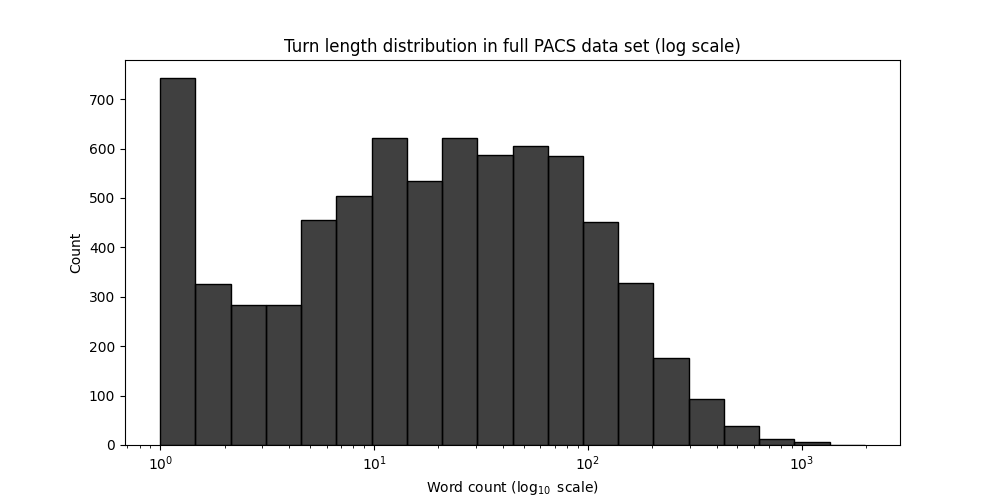
\includegraphics[width=\textwidth]{figures/log_turn_length_dist_full.png}
    \caption{Length of patient speech turns in the therapy transcripts.}
    \label{fig: PACS turn length}
\end{figure}

\begin{figure}
    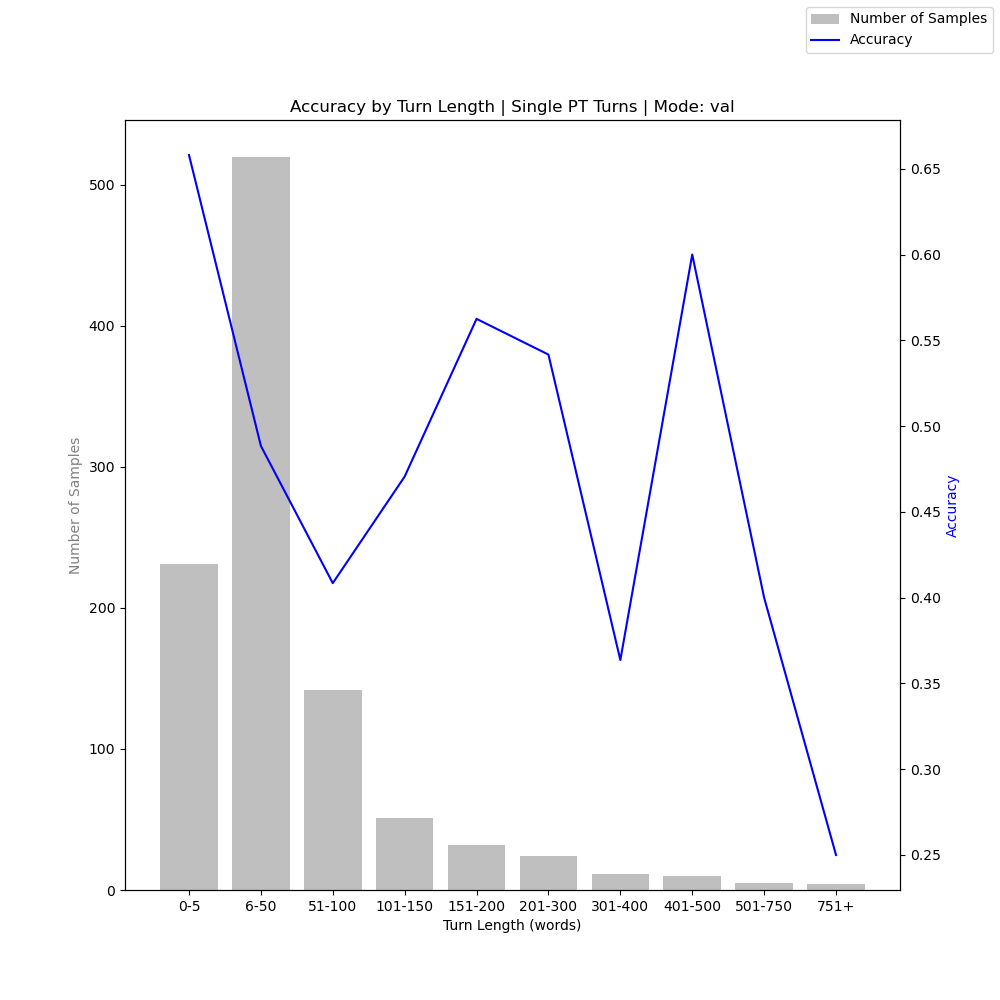
\includegraphics[width=\textwidth]{figures/accuracy_by_length_2024.03.13_11.54.44_model_7_val.png}
    \caption{Example A of accuracy over turn length for one model experiment.}
    \label{fig: acc over turn len 7}
\end{figure}

\begin{figure}
    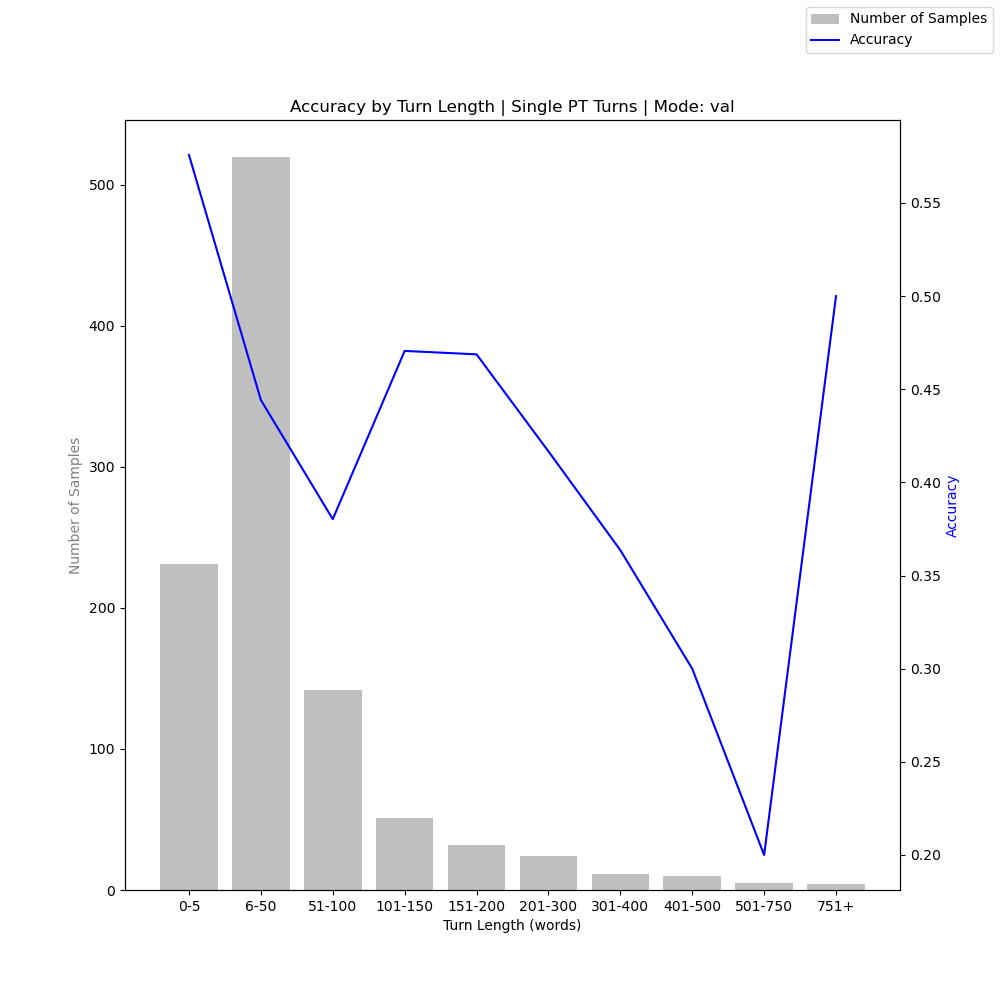
\includegraphics[width=\textwidth]{figures/accuracy_by_length_2024.03.14_09.59.35_model_11_val.png}
    \caption{Example B of accuracy over turn length for one model experiment.}
    \label{fig: acc over turn len 11}
\end{figure}

\chapter{Transformer Models}
\label{App: transformers}
At their core, the BERT and RoBERTa architectures are transformer-based models.
The transformer is a unique deep learning architecture originally demonstrated by Vaswani et al. \citeyear{Vaswani2017} for NLP purposes.
The transformer embeds an input sequence by transforming it from a sequence of $n$ symbolic representations $(x_1, \ldots, x_n)$ to a sequence of continuous representation, $z = (z_1, \ldots, z_n)$, which may then be decoded to make decisions about a down-stream task such as classifying the input.
This is achieved by first splitting the input sequence into recognised sub-words, known as tokens.
Each unique token is associated with a vocabulary ID, allowing the model to look it up in its vocabulary.
The vocabulary consists of learned vector representations of all tokens known to the model.
The vocabulary size for RoBERTa models is approximately 50,000 tokens \cite{roberta}.
Each vector represents a given token by its location in a specified dimension-space known as the embedding size.
The element values of each vocabulary vector are learned during training, so that any given embedding theoretically encodes the semantic meaning of a token in relation to other tokens.
Larger embeddings enable richer representation but comes at the cost of greater memory and computational requirements.
The embedding dimension for all BERT models, including the base RoBERTa is 768 while the large version of RoBERTa uses richer representations with dimension size 1024 \cite{BERT,roberta}.

Once the input sequence begins passing through the model, most computation is parallelised, rather than completed sequentially as was the case with previous architectures.
This is what makes training transformer models efficient and allows state-of-the-art models to process large corpora of text in their training.
To maintain the important information carried by word order despite parallel processing, the embeddings are infused with positional information through positional encoding.
This means that, following embedding and positional encoding, the model can process each token, keeping a semantic understanding of it based on its usage in the training corpus as well as knowledge of where in the sequence the token is \cite{Vaswani2017}.

What makes transformer models so powerful, however, is not only the rich embedding of positional and semantic information, but also its attention to context.
This attention mechanism allows the model to dynamically adapt its representation of tokens given their context, effectively letting each token influence all other tokens, but ensuring they only do so when relevant.
This is what allows transformer models to differentiate the financial institution from the bank of a river despite the two words having the same vocabulary ID.
More importantly, it allows the model to gain an abstract understanding of language beyond a static dictionary meaning of each word \cite{Vaswani2017}.

In transformers, attention is computed by taking the vector representation of the input sequence through three separate learned linear transformations ($W^q, W^k, W^v$), producing what are referred to as query ($q$), key ($k$), and value ($v$) reduced-dimension projections of the original embedding vectors.
The $W^q$, $W^k$, and $W^v$ weight matrices have dimension $d_{model} \times d_k$ where $d_{model}$ is the size of the input and $d_k$ is the dimension of the space the input is projected to.
In BERT-style models, including RoBERTa, $d_k = d_{model}/h$ where $d_{model}$ is the dimension of the hidden layers in the model, which is the same as the dimension of the original embeddings, 768 for base models and 1024 for the large variant of RoBERTa.
For all sizes of BERT and RoBERTa models this results in a sub-dimensional space of size 64.
Each token in any given sequence of length $n$ tokens is thus projected to three representations of size $d_k$ and the entire sequence is represented as three different matrices of shape $n \times d_k$.
Taking the dot-product of the query and key matrices and applying a softmax function to the result produces an attention mask which, when applied to the value matrix, weights all parts of the input according to how they should 'attend to' one another.
Conventionally, the dot-product of the query and key vectors is scaled by some magnitude, typically the square root of the dimension of the key vector, to avoid vanishing or exploding numbers.
Thus, the attention-mechanism in transformer models can be succinctly expressed as

$$Attention(Q,K,V) = softmax\left(\frac{QK^\intercal}{\sqrt{d_k}}\right)V$$
where $Q$, $K$, and $V$ are the matrices of stacked query ($q$), key ($k$), and value ($v$) vectors, respectively.

In most transformer models, including BERT and RoBERTa, this process occurs multiple times in parallel with different learned transformations ($W_1^q, \ldots, W_h^q, W_1^k, \ldots, W_h^k, W_1^v, \ldots, W_h^v$) corresponding to $h$ attention heads, the outputs of which are eventually concatenated into a single output and passed to a simple linear layer.
This is referred to as multi-head attention and can be expressed as
$$MultiHead(Q, K, V) = Concat(head_1, ..., head_h)W^O$$
Where, $$head_i = Attention(Q W^Q_i, K W^K_i, V W^V_i)$$
and $W^O$ is the matrix of weights in the linear layer.

While typical implementations also employ additional measures such as layer normalisation and residual connections for stability and to allow individual parts of the model to focus on learning more specific representations, the above describes the basics of the original multi-head self-attention implementation by Vaswani et al. \citeyear{Vaswani2017}.
The output of any given multi-head transformer block (encoder) may be passed as input to another transformer block or to e.g. a classification head to determine the label of the original input sequence.
The base RoBERTa architecture consists of 12 encoders each with 12 attention heads while the large RoBERTa architecture employs 24 encoders each with 16 attention heads.

\chapter{Extended Results}
\label{App: confusion matrices}

\begin{figure}
    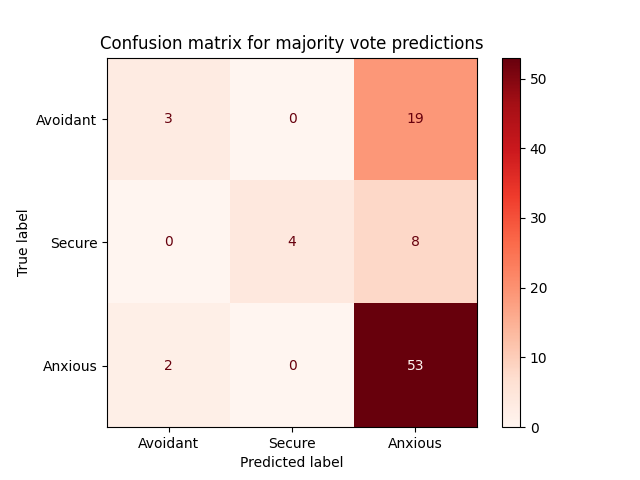
\includegraphics[width=\textwidth]{figures/roberta-large_150_combined_confusion_matrix.png}
    \caption{Confusion matrix according to majority vote classification of samples with votes from all five instances of the RoBERTa-large model trained on a minimum input length of 150 words.}
    \label{fig: combined confusion matrix}
\end{figure}

\begin{figure}
    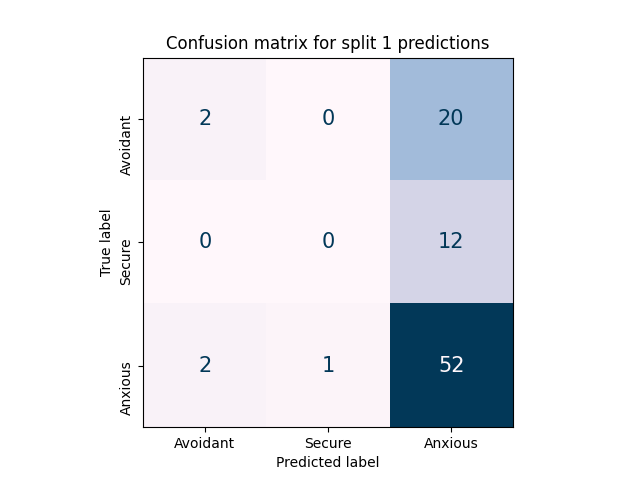
\includegraphics[width=\textwidth]{figures/roberta-large_150_split1_confusion_matrix.png}
    \caption{Confusion matrix for roberta-large model trained with minimum input length of 150 words on split 1 of the cross-validation splits.}
    \label{fig: cm split1}
\end{figure}

\begin{figure}
    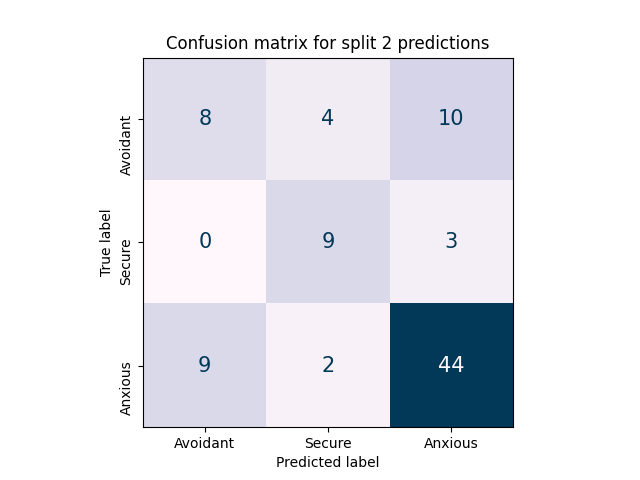
\includegraphics[width=\textwidth]{figures/roberta-large_150_split2_confusion_matrix.png}
    \caption{Confusion matrix for roberta-large model trained with minimum input length of 150 words on split 2 of the cross-validation splits.}
    \label{fig: cm split2}
\end{figure}

\begin{figure}
    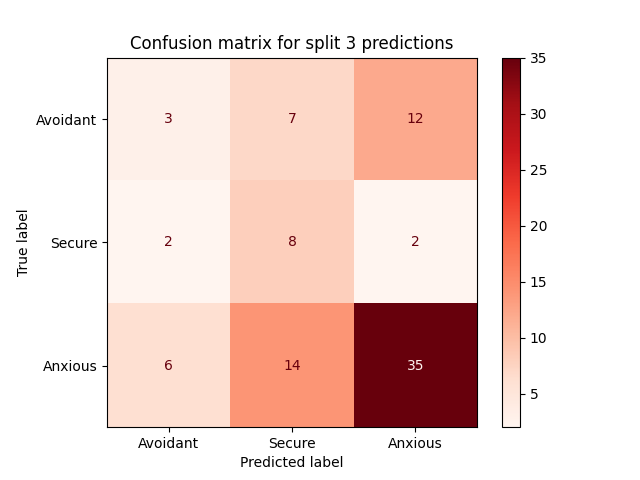
\includegraphics[width=\textwidth]{figures/roberta-large_150_split3_confusion_matrix.png}
    \caption{Confusion matrix for roberta-large model trained with minimum input length of 150 words on split 3 of the cross-validation splits.}
    \label{fig: cm split3}
\end{figure}

\begin{figure}
    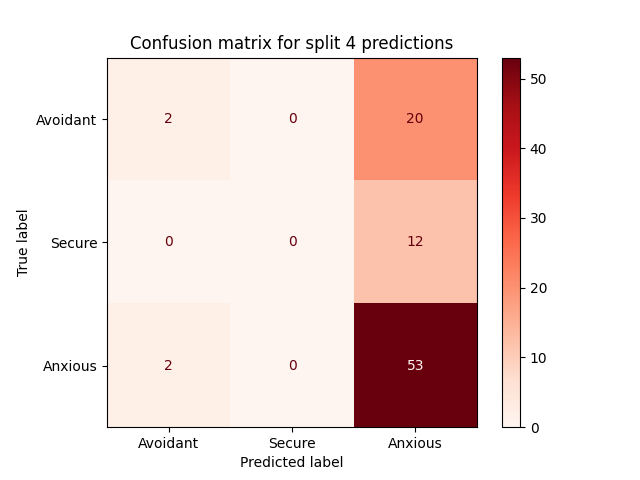
\includegraphics[width=\textwidth]{figures/roberta-large_150_split4_confusion_matrix.png}
    \caption{Confusion matrix for roberta-large model trained with minimum input length of 150 words on split 4 of the cross-validation splits.}
    \label{fig: cm split4}
\end{figure}

\begin{figure}
    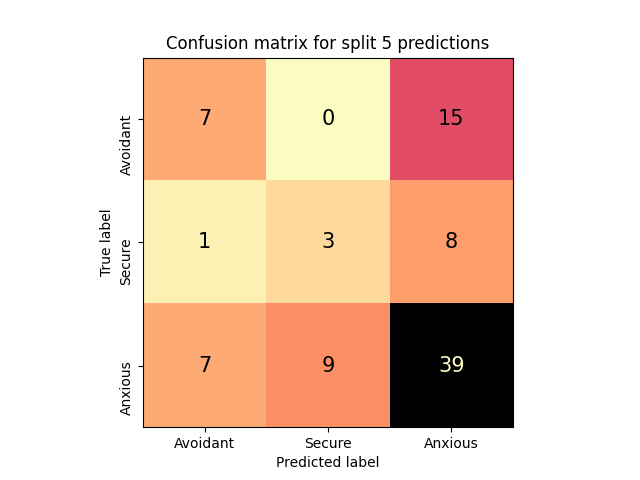
\includegraphics[width=\textwidth]{figures/roberta-large_150_split5_confusion_matrix.png}
    \caption{Confusion matrix for roberta-large model trained with minimum input length of 150 words on split 5 of the cross-validation splits.}
    \label{fig: cm split5}
\end{figure}
    
\end{document}